\subsection{Trigonometric Functions from Euclidean Geometry}

\begin{remark*}[Geometric intuition]
A right triangle fixes three side lengths relative to an acute angle:
opposite, adjacent, and hypotenuse. Similar right triangles may be larger or
smaller, but their corresponding side ratios are unchanged. This invariance is
what makes a trigonometric ratio a function of the angle rather than a feature
of one drawing.
\end{remark*}

\begin{center}
\begin{tikzpicture}[scale=1.25, line cap=round, line join=round]
  \definecolor{trigblue}{RGB}{30,110,190}
  \coordinate (A) at (0,0);
  \coordinate (B) at (3.4,0);
  \coordinate (C) at (3.4,2.0);
  \draw[very thick] (A)--(B)--(C)--cycle;
  \draw (3.1,0)--(3.1,0.3)--(3.4,0.3);
  \draw[trigblue] (0.55,0) arc[start angle=0,end angle=30.5,radius=0.55];
  \node[trigblue] at (0.78,0.22) {$\theta$};
  \node[below] at ($(A)!0.5!(B)$) {adjacent};
  \node[right] at ($(B)!0.5!(C)$) {opposite};
  \node[above left] at ($(A)!0.5!(C)$) {hypotenuse};
  \foreach \p/\pos in {A/below left,B/below right,C/above right}{
    \fill (\p) circle (0.025);
    \node[\pos] at (\p) {$\p$};
  }
\end{tikzpicture}
\end{center}


\begin{remark*}[Primitive and derived ratios]
The primitive geometric ratios are sine and cosine. Tangent, cotangent, secant,
and cosecant are convenient quotient or reciprocal ratios built from the same
three side lengths.
\end{remark*}
\begin{dependencies}
\begin{itemize}
  \item \hyperref[def:euclid-triangle-angle-classes]{Right-angled triangle}
  \item \hyperref[def:euclid-right-angle-and-perpendicular]{Right angle and perpendicular}
\end{itemize}
\end{dependencies}

\begin{center}
\begin{tikzpicture}[scale=1.25, line cap=round, line join=round]
  \definecolor{trigblue}{RGB}{30,110,190}
  \coordinate (A) at (0,0);
  \coordinate (B) at (3.4,0);
  \coordinate (C) at (3.4,2.0);
  \draw[very thick] (A)--(B)--(C)--cycle;
  \draw[line width=2.1pt,trigblue] (A)--(B);
  \draw[line width=2.1pt,trigblue] (B)--(C);
  \draw[line width=2.1pt,gray!65] (A)--(C);
  \draw (3.1,0)--(3.1,0.3)--(3.4,0.3);
  \draw[trigblue] (0.55,0) arc[start angle=0,end angle=30.5,radius=0.55];
  \node[trigblue] at (0.78,0.22) {$\theta$};
  \node[below,trigblue] at ($(A)!0.5!(B)$) {$\cos\theta$ side};
  \node[right,trigblue] at ($(B)!0.5!(C)$) {$\sin\theta$ side};
  \node[above left] at ($(A)!0.5!(C)$) {hypotenuse};
\end{tikzpicture}
\end{center}


\begin{definitionbox}{Definition}
\begin{definition}[Right-triangle sine]
\label{def:right-triangle-sine}
Let $T$ be a right triangle and let $\theta$ be one of its acute angles. Write
\[
  \operatorname{opp}(T,\theta),\qquad
  \operatorname{adj}(T,\theta),\qquad
  \operatorname{hyp}(T)
\]
for the side lengths opposite $\theta$, adjacent to $\theta$, and opposite the
right angle, respectively. Define
\[
\sin\theta=\frac{\operatorname{opp}(T,\theta)}{\operatorname{hyp}(T)}.
\]
\end{definition}
\end{definitionbox}
\begin{dependencies}
\begin{itemize}
  \item \hyperref[def:euclid-triangle-angle-classes]{Right-angled triangle}
  \item \hyperref[def:euclid-right-angle-and-perpendicular]{Right angle and perpendicular}
  \item \hyperref[def:euclid-acute-angle]{Acute angle}
\end{itemize}
\end{dependencies}

\begin{definitionbox}{Definition}
\begin{definition}[Acute-angle sine]
\label{def:acute-angle-sine}
For an acute Euclidean angle $\theta$, choose any right triangle $T$ having
$\theta$ as an acute angle and set
\[
  \sin\theta=\frac{\operatorname{opp}(T,\theta)}{\operatorname{hyp}(T)}.
\]
\end{definition}
\end{definitionbox}
\begin{dependencies}
\begin{itemize}
  \item \hyperref[def:right-triangle-sine]{Right-triangle sine}
  \item \hyperref[thm:trig-ratios-similarity-invariant]{Similarity invariance of trigonometric ratios}
\end{itemize}
\end{dependencies}

\begin{center}
\begin{tikzpicture}[scale=1.55, line cap=round, line join=round]
  \definecolor{trigblue}{RGB}{30,110,190}
  \coordinate (O) at (0,0);
  \coordinate (P) at (35:1);
  \coordinate (Q) at ({cos(35)},0);
  \draw[gray!55] (O) circle (1);
  \draw[->] (-1.25,0)--(1.35,0) node[right] {$x$};
  \draw[->] (0,-1.15)--(0,1.25) node[above] {$y$};
  \draw[very thick, trigblue] (Q)--(P);
  \draw[very thick] (O)--(P);
  \draw[dropline] (P)--(Q);
  \draw[trigblue] (0.32,0) arc[start angle=0,end angle=35,radius=0.32];
  \node[trigblue] at (0.32,0.10) {$\theta$};
  \fill (P) circle (0.022) node[above right] {$P=(x_\theta,y_\theta)$};
  \node[right,trigblue] at ($(Q)!0.5!(P)$) {$\sin\theta=y_\theta$};
\end{tikzpicture}
\end{center}


\begin{definitionbox}{Definition}
\begin{definition}[Unit-circle sine]
\label{def:unit-circle-sine}
Let $\theta$ be an angle in standard position, and let $P(\theta)=(x_\theta,
y_\theta)$ be the point where its terminal ray meets the unit circle. Define
\[
  \sin\theta=y_\theta.
\]
\end{definition}
\end{definitionbox}
\begin{dependencies}
\begin{itemize}
  \item \hyperref[def:euclid-circle]{Circle}
  \item \hyperref[def:cartesian-product]{Cartesian Product}
\end{itemize}
\end{dependencies}

\begin{center}
\begin{tikzpicture}[scale=1.25, line cap=round, line join=round]
  \definecolor{trigblue}{RGB}{30,110,190}
  \coordinate (A) at (0,0);
  \coordinate (B) at (3.4,0);
  \coordinate (C) at (3.4,2.0);
  \draw[very thick] (A)--(B)--(C)--cycle;
  \draw[line width=2.2pt,trigblue] (A)--(B);
  \draw[line width=2.2pt,gray!65] (A)--(C);
  \draw (3.1,0)--(3.1,0.3)--(3.4,0.3);
  \draw[trigblue] (0.55,0) arc[start angle=0,end angle=30.5,radius=0.55];
  \node[trigblue] at (0.78,0.22) {$\theta$};
  \node[below,trigblue] at ($(A)!0.5!(B)$) {adjacent};
  \node[above left] at ($(A)!0.5!(C)$) {hypotenuse};
  \node[below] at (1.7,-0.55) {$\cos\theta=\text{adjacent}/\text{hypotenuse}$};
\end{tikzpicture}
\end{center}


\begin{definitionbox}{Definition}
\begin{definition}[Right-triangle cosine]
\label{def:right-triangle-cosine}
Let $T$ be a right triangle and let $\theta$ be one of its acute angles. Define
\[
\cos\theta=\frac{\operatorname{adj}(T,\theta)}{\operatorname{hyp}(T)}.
\]
\end{definition}
\end{definitionbox}

\begin{center}
\begin{tikzpicture}[scale=1.25, line cap=round, line join=round]
  \definecolor{trigblue}{RGB}{30,110,190}
  \coordinate (A) at (0,0);
  \coordinate (B) at (3.4,0);
  \coordinate (C) at (3.4,2.0);
  \draw[very thick] (A)--(B)--(C)--cycle;
  \draw[line width=2.1pt,trigblue] (A)--(B);
  \draw[line width=2.1pt,gray!65] (A)--(C);
  \draw (3.1,0)--(3.1,0.3)--(3.4,0.3);
  \draw[trigblue] (0.55,0) arc[start angle=0,end angle=30.5,radius=0.55];
  \node[trigblue] at (0.78,0.22) {$\theta$};
  \node[below,trigblue] at ($(A)!0.5!(B)$) {$\operatorname{adj}(T,\theta)$};
  \node[above left] at ($(A)!0.5!(C)$) {$\operatorname{hyp}(T)$};
  \node[below] at (1.7,-0.55) {$\cos\theta=\operatorname{adj}(T,\theta)/\operatorname{hyp}(T)$};
\end{tikzpicture}
\end{center}


\begin{definitionbox}{Definition}
\begin{definition}[Acute-angle cosine]
\label{def:acute-angle-cosine}
For an acute Euclidean angle $\theta$, choose any right triangle $T$ having
$\theta$ as an acute angle and set
\[
  \cos\theta=\frac{\operatorname{adj}(T,\theta)}{\operatorname{hyp}(T)}.
\]
\end{definition}
\end{definitionbox}

\begin{center}
\begin{tikzpicture}[scale=1.55, line cap=round, line join=round]
  \definecolor{trigblue}{RGB}{30,110,190}
  \coordinate (O) at (0,0);
  \coordinate (P) at (35:1);
  \coordinate (Q) at ({cos(35)},0);
  \draw[gray!55] (O) circle (1);
  \draw[->] (-1.25,0)--(1.35,0) node[right] {$x$};
  \draw[->] (0,-1.15)--(0,1.25) node[above] {$y$};
  \draw[very thick, trigblue] (O)--(P);
  \draw[very thick] (Q)--(P);
  \draw[very thick] (O)--(Q);
  \draw (Q)+(-0.12,0)--++(0,0.12)--++(0.12,0);
  \draw[trigblue] (0.32,0) arc[start angle=0,end angle=35,radius=0.32];
  \node[trigblue] at (0.32,0.10) {$\theta$};
  \fill (O) circle (0.018) node[below left] {$O$};
  \fill (P) circle (0.022) node[above right] {$P(\theta)=(\cos\theta,\sin\theta)$};
  \node[below] at ($(O)!0.5!(Q)$) {$\cos\theta$};
  \node[right] at ($(Q)!0.5!(P)$) {$\sin\theta$};
\end{tikzpicture}
\end{center}


\begin{definitionbox}{Definition}
\begin{definition}[Unit-circle cosine]
\label{def:unit-circle-cosine}
Let $\theta$ be an angle in standard position, and let $P(\theta)=(x_\theta,
y_\theta)$ be the point where its terminal ray meets the unit circle. Define
\[
  \cos\theta=x_\theta.
\]
\end{definition}
\end{definitionbox}

\begin{center}
\begin{tikzpicture}[scale=1.25, line cap=round, line join=round]
  \definecolor{trigblue}{RGB}{30,110,190}
  \coordinate (A) at (0,0);
  \coordinate (B) at (3.4,0);
  \coordinate (C) at (3.4,2.0);
  \draw[very thick] (A)--(B)--(C)--cycle;
  \draw[line width=2.2pt,trigblue] (B)--(C);
  \draw[line width=2.2pt,gray!65] (A)--(B);
  \draw (3.1,0)--(3.1,0.3)--(3.4,0.3);
  \draw[trigblue] (0.55,0) arc[start angle=0,end angle=30.5,radius=0.55];
  \node[trigblue] at (0.78,0.22) {$\theta$};
  \node[right,trigblue] at ($(B)!0.5!(C)$) {opposite};
  \node[below] at ($(A)!0.5!(B)$) {adjacent};
  \node[below] at (1.7,-0.55) {$\tan\theta=\text{opposite}/\text{adjacent}$};
\end{tikzpicture}
\end{center}


\begin{definitionbox}{Definition}
\begin{definition}[Right-triangle tangent]
\label{def:right-triangle-tangent}
Let $T$ be a right triangle and let $\theta$ be one of its acute angles. Define
\[
\tan\theta=\frac{\operatorname{opp}(T,\theta)}{\operatorname{adj}(T,\theta)}.
\]
\end{definition}
\end{definitionbox}

\begin{center}
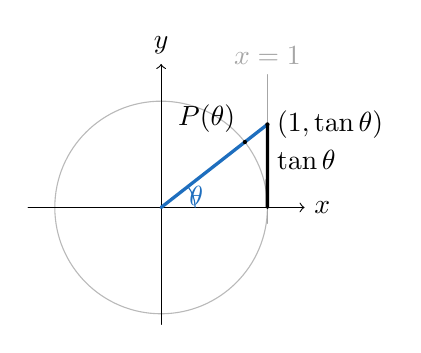
\begin{tikzpicture}[scale=1.35, line cap=round, line join=round]
  \definecolor{trigblue}{RGB}{30,110,190}
  \coordinate (O) at (0,0);
  \coordinate (P) at (38:1);
  \coordinate (T) at (1,{tan(38)});
  \draw[gray!55] (O) circle (1);
  \draw[->] (-1.25,0)--(1.35,0) node[right] {$x$};
  \draw[->] (0,-1.1)--(0,1.35) node[above] {$y$};
  \draw[gray!70] (1,-0.15)--(1,1.25) node[above] {$x=1$};
  \draw[very thick, trigblue] (O)--(T);
  \draw[very thick] (1,0)--(T);
  \fill (P) circle (0.02) node[above left] {$P(\theta)$};
  \fill (T) circle (0.02) node[right] {$(1,\tan\theta)$};
  \node[right] at (1,0.45) {$\tan\theta$};
  \draw[trigblue] (0.32,0) arc[start angle=0,end angle=38,radius=0.32];
  \node[trigblue] at (0.33,0.11) {$\theta$};
\end{tikzpicture}
\end{center}


\begin{definitionbox}{Definition}
\begin{definition}[Extended tangent]
\label{def:extended-tangent}
Where $\cos\theta\neq 0$, define
\[
  \tan\theta=\frac{\sin\theta}{\cos\theta}.
\]
\end{definition}
\end{definitionbox}
\begin{remark*}[Geometric reading]
The tangent of $\theta$ is the signed height where the terminal ray meets the
vertical tangent line $x=1$.
\end{remark*}

\input{volume-i/book-geometry/trigonometry/foundations/figure-right-triangle-cotangent}

\begin{definitionbox}{Definition}
\begin{definition}[Right-triangle cotangent]
\label{def:right-triangle-cotangent}
Let $T$ be a right triangle and let $\theta$ be one of its acute angles. Define
\[
\cot\theta=\frac{\operatorname{adj}(T,\theta)}{\operatorname{opp}(T,\theta)}.
\]
\end{definition}
\end{definitionbox}

\begin{center}
\begin{tikzpicture}[scale=1.3, line cap=round, line join=round]
  \definecolor{trigblue}{RGB}{30,110,190}
  \coordinate (O) at (0,0);
  \coordinate (T) at ({cot(38)},1);
  \draw[gray!55] (O) circle (1);
  \draw[->] (-0.2,0)--(1.55,0) node[right] {$x$};
  \draw[->] (0,-0.2)--(0,1.35) node[above] {$y$};
  \draw[gray!70] (-0.15,1)--(1.35,1) node[right] {$y=1$};
  \draw[very thick,trigblue] (O)--(T);
  \draw[very thick] (0,1)--(T);
  \fill (T) circle (0.02) node[above] {$(\cot\theta,1)$};
  \node[above] at ($(0,1)!0.5!(T)$) {$\cot\theta$};
\end{tikzpicture}
\end{center}


\begin{definitionbox}{Definition}
\begin{definition}[Extended cotangent]
\label{def:extended-cotangent}
Where $\sin\theta\neq 0$, define
\[
  \cot\theta=\frac{\cos\theta}{\sin\theta}.
\]
\end{definition}
\end{definitionbox}

\input{volume-i/book-geometry/trigonometry/foundations/figure-right-triangle-secant}

\begin{definitionbox}{Definition}
\begin{definition}[Right-triangle secant]
\label{def:right-triangle-secant}
Let $T$ be a right triangle and let $\theta$ be one of its acute angles. Define
\[
\sec\theta=\frac{\operatorname{hyp}(T)}{\operatorname{adj}(T,\theta)}.
\]
\end{definition}
\end{definitionbox}

\begin{center}
\begin{tikzpicture}[scale=1.35, line cap=round, line join=round]
  \definecolor{trigblue}{RGB}{30,110,190}
  \coordinate (O) at (0,0);
  \coordinate (T) at (1,{tan(38)});
  \draw[gray!55] (O) circle (1);
  \draw[->] (-0.25,0)--(1.35,0) node[right] {$x$};
  \draw[->] (0,-0.2)--(0,1.35) node[above] {$y$};
  \draw[gray!70] (1,-0.1)--(1,1.25) node[above] {$x=1$};
  \draw[very thick,trigblue] (O)--(T);
  \fill (T) circle (0.02) node[right] {$(1,\tan\theta)$};
  \node[above left,trigblue] at ($(O)!0.52!(T)$) {$\sec\theta$};
\end{tikzpicture}
\end{center}


\begin{definitionbox}{Definition}
\begin{definition}[Extended secant]
\label{def:extended-secant}
Where $\cos\theta\neq 0$, define
\[
  \sec\theta=\frac{1}{\cos\theta}.
\]
\end{definition}
\end{definitionbox}

\begin{center}
\begin{tikzpicture}[scale=1.25, line cap=round, line join=round]
  \definecolor{trigblue}{RGB}{30,110,190}
  \coordinate (A) at (0,0);
  \coordinate (B) at (3.4,0);
  \coordinate (C) at (3.4,2.0);
  \draw[very thick] (A)--(B)--(C)--cycle;
  \draw[line width=2.2pt,trigblue] (A)--(C);
  \draw[line width=2.2pt,gray!65] (B)--(C);
  \draw (3.1,0)--(3.1,0.3)--(3.4,0.3);
  \draw[trigblue] (0.55,0) arc[start angle=0,end angle=30.5,radius=0.55];
  \node[trigblue] at (0.78,0.22) {$\theta$};
  \node[above left,trigblue] at ($(A)!0.5!(C)$) {hypotenuse};
  \node[right] at ($(B)!0.5!(C)$) {opposite};
  \node[below] at (1.7,-0.55) {$\csc\theta=\text{hypotenuse}/\text{opposite}$};
\end{tikzpicture}
\end{center}


\begin{definitionbox}{Definition}
\begin{definition}[Right-triangle cosecant]
\label{def:right-triangle-cosecant}
Let $T$ be a right triangle and let $\theta$ be one of its acute angles. Define
\[
\csc\theta=\frac{\operatorname{hyp}(T)}{\operatorname{opp}(T,\theta)}.
\]
\end{definition}
\end{definitionbox}
\begin{remark*}[Standard quantified statement]
For every admissible input satisfying the hypotheses of the statement, the
displayed definition or assertion holds in the stated domain.
\end{remark*}

\begin{remark*}[Interpretation]
The statement records the named trigonometric object or identity together with
its intended domain of use.
\end{remark*}

\begin{dependencies}
\begin{itemize}
  \item \hyperref[def:euclid-triangle-angle-classes]{Right-angled triangle}
  \item \hyperref[def:euclid-right-angle-and-perpendicular]{Right angle and perpendicular}
  \item \hyperref[def:euclid-acute-angle]{Acute angle}
\end{itemize}
\end{dependencies}

\input{volume-i/book-geometry/trigonometry/foundations/figure-extended-cosecant}

\begin{definitionbox}{Definition}
\begin{definition}[Extended cosecant]
\label{def:extended-cosecant}
Where $\sin\theta\neq 0$, define
\[
  \csc\theta=\frac{1}{\sin\theta}.
\]
\end{definition}
\end{definitionbox}
\begin{remark*}[Standard quantified statement]
For every admissible input satisfying the hypotheses of the statement, the
displayed definition or assertion holds in the stated domain.
\end{remark*}

\begin{remark*}[Interpretation]
The statement records the named trigonometric object or identity together with
its intended domain of use.
\end{remark*}

\begin{dependencies}
\begin{itemize}
  \item \hyperref[def:unit-circle-sine]{Unit-circle sine}
\end{itemize}
\end{dependencies}

\begin{center}
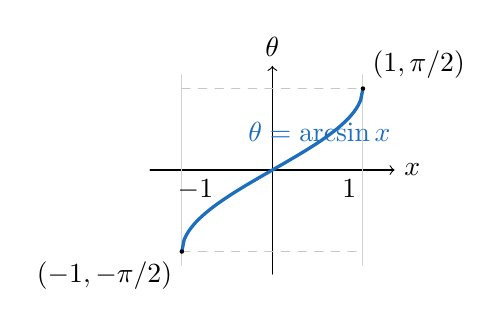
\begin{tikzpicture}[scale=1.15, line cap=round, line join=round]
  \definecolor{trigblue}{RGB}{30,110,190}
  \draw[->] (-1.35,0)--(1.35,0) node[right] {$x$};
  \draw[->] (0,-1.15)--(0,1.15) node[above] {$\theta$};
  \draw[gray!35] (-1,-1.05)--(-1,1.05);
  \draw[gray!35] (1,-1.05)--(1,1.05);
  \draw[gray!45,dashed] (-1,-0.9)--(1,-0.9);
  \draw[gray!45,dashed] (-1,0.9)--(1,0.9);
  \draw[very thick,trigblue,domain=-1:1,samples=80]
    plot ({\x},{0.9*asin(\x)/90});
  \fill (-1,-0.9) circle (0.025) node[below left] {$(-1,-\pi/2)$};
  \fill (1,0.9) circle (0.025) node[above right] {$(1,\pi/2)$};
  \node[trigblue] at (0.52,0.42) {$\theta=\arcsin x$};
  \node[below] at (0.85,0) {$1$};
  \node[below] at (-0.85,0) {$-1$};
\end{tikzpicture}
\end{center}


\begin{definitionbox}{Definition}
\begin{definition}[Inverse sine]
\label{def:inverse-sine}
The \emph{inverse sine} function is the inverse of sine after sine is
restricted to the interval
\[
  \left[-\frac{\pi}{2},\frac{\pi}{2}\right].
\]
It is denoted by $\arcsin$ or $\sin^{-1}$ and has domain $[-1,1]$ and range
$[-\pi/2,\pi/2]$.
\[
  \arcsin x=\theta
  \quad\Longleftrightarrow\quad
  \sin\theta=x
  \quad\text{and}\quad
  -\frac{\pi}{2}\leq\theta\leq\frac{\pi}{2}.
\]
\end{definition}
\end{definitionbox}
\begin{remark*}[Domain and range]
The full sine function has domain all real-valued angle measures and range
$[-1,1]$. The inverse sine function reverses the restricted sine function, so
its domain is $[-1,1]$ and its range is the principal interval
$[-\pi/2,\pi/2]$.
\end{remark*}
\begin{dependencies}
\begin{itemize}
  \item \hyperref[def:unit-circle-sine]{Unit-circle sine}
  \item \hyperref[def:radian-measure]{Radian measure}
\end{itemize}
\end{dependencies}

\begin{theorembox}{Theorem}
\begin{theorem}[Principal inverse sine identities]
\label{thm:inverse-sine-identities}
For every $x\in[-1,1]$,
\[
  \sin(\arcsin x)=x.
\]
For every $\theta\in[-\pi/2,\pi/2]$,
\[
  \arcsin(\sin\theta)=\theta.
\]
\end{theorem}
\end{theorembox}
\begin{remark*}[Standard quantified statement]
\[
  \forall x\in[-1,1],\quad \sin(\arcsin x)=x,
  \qquad
  \forall \theta\in[-\pi/2,\pi/2],\quad \arcsin(\sin\theta)=\theta.
\]
\end{remark*}
\begin{dependencies}
\begin{itemize}
  \item \hyperref[def:inverse-sine]{Inverse sine}
\end{itemize}
\end{dependencies}

\begin{center}
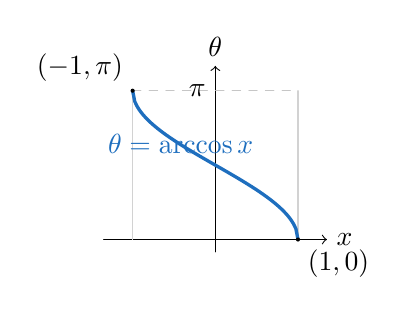
\begin{tikzpicture}[scale=1.05, line cap=round, line join=round]
  \definecolor{trigblue}{RGB}{30,110,190}
  \draw[->] (-1.35,0)--(1.35,0) node[right] {$x$};
  \draw[->] (0,-0.15)--(0,2.1) node[above] {$\theta$};
  \draw[gray!35] (-1,0)--(-1,1.8);
  \draw[gray!35] (1,0)--(1,1.8);
  \draw[gray!45,dashed] (-1,1.8)--(1,1.8);
  \draw[very thick,trigblue,domain=-1:1,samples=80]
    plot ({\x},{1.8*acos(\x)/180});
  \fill (-1,1.8) circle (0.025) node[above left] {$(-1,\pi)$};
  \fill (1,0) circle (0.025) node[below right] {$(1,0)$};
  \node[trigblue] at (-0.42,1.16) {$\theta=\arccos x$};
  \node[left] at (0,1.8) {$\pi$};
\end{tikzpicture}
\end{center}


\begin{definitionbox}{Definition}
\begin{definition}[Inverse cosine]
\label{def:inverse-cosine}
The \emph{inverse cosine} function is the inverse of cosine after cosine is
restricted to the interval $[0,\pi]$. It is denoted by $\arccos$ or
$\cos^{-1}$ and has domain $[-1,1]$ and range $[0,\pi]$.
\[
  \arccos x=\theta
  \quad\Longleftrightarrow\quad
  \cos\theta=x
  \quad\text{and}\quad
  0\leq\theta\leq\pi.
\]
\end{definition}
\end{definitionbox}
\begin{remark*}[Standard quantified statement]
For every admissible input satisfying the hypotheses of the statement, the
displayed definition or assertion holds in the stated domain.
\end{remark*}

\begin{remark*}[Interpretation]
The statement records the named trigonometric object or identity together with
its intended domain of use.
\end{remark*}

\begin{remark*}[Domain and range]
The full cosine function has domain all real-valued angle measures and range
$[-1,1]$. The inverse cosine function reverses the restricted cosine function,
so its domain is $[-1,1]$ and its range is the principal interval $[0,\pi]$.
\end{remark*}
\begin{dependencies}
\begin{itemize}
  \item \hyperref[def:unit-circle-cosine]{Unit-circle cosine}
  \item \hyperref[def:radian-measure]{Radian measure}
\end{itemize}
\end{dependencies}

\begin{theorembox}{Theorem}
\begin{theorem}[Principal inverse cosine identities]
\label{thm:inverse-cosine-identities}
For every $x\in[-1,1]$,
\[
  \cos(\arccos x)=x.
\]
For every $\theta\in[0,\pi]$,
\[
  \arccos(\cos\theta)=\theta.
\]
\end{theorem}
\end{theorembox}
\begin{remark*}[Interpretation]
The statement records the named trigonometric object or identity together with
its intended domain of use.
\end{remark*}

\begin{remark*}[Standard quantified statement]
$\forall x\in[-1,1]$, $\cos(\arccos x)=x$, and
$\forall \theta\in[0,\pi]$, $\arccos(\cos\theta)=\theta$.
\end{remark*}
\begin{dependencies}
\begin{itemize}
  \item \hyperref[def:inverse-cosine]{Inverse cosine}
\end{itemize}
\end{dependencies}

\begin{center}
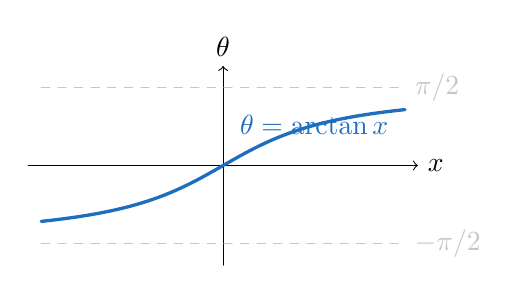
\begin{tikzpicture}[scale=1.1, line cap=round, line join=round]
  \definecolor{trigblue}{RGB}{30,110,190}
  \draw[->] (-2.25,0)--(2.25,0) node[right] {$x$};
  \draw[->] (0,-1.15)--(0,1.15) node[above] {$\theta$};
  \draw[gray!45,dashed] (-2.1,0.9)--(2.1,0.9) node[right] {$\pi/2$};
  \draw[gray!45,dashed] (-2.1,-0.9)--(2.1,-0.9) node[right] {$-\pi/2$};
  \draw[very thick,trigblue,domain=-2.1:2.1,samples=90]
    plot ({\x},{0.9*atan(\x)/90});
  \node[trigblue] at (1.05,0.47) {$\theta=\arctan x$};
\end{tikzpicture}
\end{center}


\begin{definitionbox}{Definition}
\begin{definition}[Inverse tangent]
\label{def:inverse-tangent}
The \emph{inverse tangent} function is the inverse of tangent after tangent is
restricted to the interval $(-\pi/2,\pi/2)$. It is denoted by $\arctan$ or
$\tan^{-1}$ and has domain $\mathbb{R}$ and range $(-\pi/2,\pi/2)$.
\[
  \arctan x=\theta
  \quad\Longleftrightarrow\quad
  \tan\theta=x
  \quad\text{and}\quad
  -\frac{\pi}{2}<\theta<\frac{\pi}{2}.
\]
\end{definition}
\end{definitionbox}
\begin{remark*}[Standard quantified statement]
For every admissible input satisfying the hypotheses of the statement, the
displayed definition or assertion holds in the stated domain.
\end{remark*}

\begin{remark*}[Interpretation]
The statement records the named trigonometric object or identity together with
its intended domain of use.
\end{remark*}

\begin{remark*}[Domain and range]
The tangent function has domain
$\mathbb{R}\setminus\{\pi/2+k\pi:k\in\mathbb{Z}\}$ and range $\mathbb{R}$.
The inverse tangent function reverses the principal restricted tangent
function, so its domain is $\mathbb{R}$ and its range is
$(-\pi/2,\pi/2)$.
\end{remark*}
\begin{dependencies}
\begin{itemize}
  \item \hyperref[def:extended-tangent]{Extended tangent}
  \item \hyperref[def:radian-measure]{Radian measure}
\end{itemize}
\end{dependencies}

\begin{theorembox}{Theorem}
\begin{theorem}[Principal inverse tangent identities]
\label{thm:inverse-tangent-identities}
For every $x\in\mathbb{R}$,
\[
  \tan(\arctan x)=x.
\]
For every $\theta\in(-\pi/2,\pi/2)$,
\[
  \arctan(\tan\theta)=\theta.
\]
\end{theorem}
\end{theorembox}
\begin{remark*}[Interpretation]
The statement records the named trigonometric object or identity together with
its intended domain of use.
\end{remark*}

\begin{remark*}[Standard quantified statement]
$\forall x\in\mathbb{R}$, $\tan(\arctan x)=x$, and
$\forall \theta\in(-\pi/2,\pi/2)$, $\arctan(\tan\theta)=\theta$.
\end{remark*}
\begin{dependencies}
\begin{itemize}
  \item \hyperref[def:inverse-tangent]{Inverse tangent}
\end{itemize}
\end{dependencies}

\begin{center}
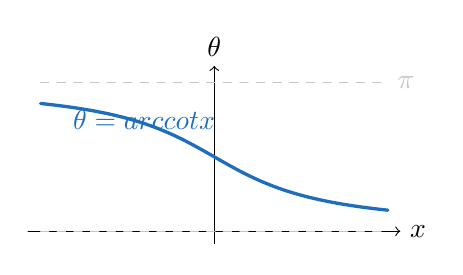
\begin{tikzpicture}[scale=1.05, line cap=round, line join=round]
  \definecolor{trigblue}{RGB}{30,110,190}
  \draw[->] (-2.25,0)--(2.25,0) node[right] {$x$};
  \draw[->] (0,-0.15)--(0,2.0) node[above] {$\theta$};
  \draw[gray!45,dashed] (-2.1,1.8)--(2.1,1.8) node[right] {$\pi$};
  \draw[gray!45,dashed] (-2.1,0)--(2.1,0);
  \draw[very thick,trigblue,domain=-2.1:2.1,samples=90]
    plot ({\x},{0.9+0.9*(-atan(\x)/90)});
  \node[trigblue] at (-0.85,1.35) {$\theta=\operatorname{arccot} x$};
\end{tikzpicture}
\end{center}


\begin{definitionbox}{Definition}
\begin{definition}[Inverse cotangent]
\label{def:inverse-cotangent}
The \emph{inverse cotangent} function is the inverse of cotangent after
cotangent is restricted to the interval $(0,\pi)$. It is denoted by $\operatorname{arccot}$
or $\cot^{-1}$ and has domain $\mathbb{R}$ and range $(0,\pi)$.
\[
  \operatorname{arccot} x=\theta
  \quad\Longleftrightarrow\quad
  \cot\theta=x
  \quad\text{and}\quad
  0<\theta<\pi.
\]
\end{definition}
\end{definitionbox}
\begin{remark*}[Domain and range]
The cotangent function has domain
$\mathbb{R}\setminus\{k\pi:k\in\mathbb{Z}\}$ and range $\mathbb{R}$. The
inverse cotangent function reverses the principal restricted cotangent
function, so its domain is $\mathbb{R}$ and its range is $(0,\pi)$.
\end{remark*}
\begin{dependencies}
\begin{itemize}
  \item \hyperref[def:extended-cotangent]{Extended cotangent}
  \item \hyperref[def:radian-measure]{Radian measure}
\end{itemize}
\end{dependencies}

\begin{theorembox}{Theorem}
\begin{theorem}[Principal inverse cotangent identities]
\label{thm:inverse-cotangent-identities}
For every $x\in\mathbb{R}$,
\[
  \cot(\operatorname{arccot} x)=x.
\]
For every $\theta\in(0,\pi)$,
\[
  \operatorname{arccot}(\cot\theta)=\theta.
\]
\end{theorem}
\end{theorembox}
\begin{remark*}[Standard quantified statement]
$\forall x\in\mathbb{R}$, $\cot(\operatorname{arccot} x)=x$, and
$\forall \theta\in(0,\pi)$, $\operatorname{arccot}(\cot\theta)=\theta$.
\end{remark*}
\begin{dependencies}
\begin{itemize}
  \item \hyperref[def:inverse-cotangent]{Inverse cotangent}
\end{itemize}
\end{dependencies}

\begin{center}
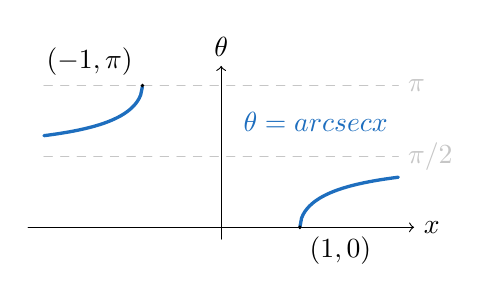
\begin{tikzpicture}[scale=1.0, line cap=round, line join=round]
  \definecolor{trigblue}{RGB}{30,110,190}
  \draw[->] (-2.45,0)--(2.45,0) node[right] {$x$};
  \draw[->] (0,-0.15)--(0,2.05) node[above] {$\theta$};
  \draw[gray!45,dashed] (-2.25,1.8)--(2.25,1.8) node[right] {$\pi$};
  \draw[gray!45,dashed] (-2.25,0.9)--(2.25,0.9) node[right] {$\pi/2$};
  \draw[very thick,trigblue,domain=1:2.25,samples=60]
    plot ({\x},{1.8*acos(1/\x)/180});
  \draw[very thick,trigblue,domain=-2.25:-1,samples=60]
    plot ({\x},{1.8*acos(1/\x)/180});
  \fill (1,0) circle (0.025) node[below right] {$(1,0)$};
  \fill (-1,1.8) circle (0.025) node[above left] {$(-1,\pi)$};
  \node[trigblue] at (1.2,1.34) {$\theta=\operatorname{arcsec} x$};
\end{tikzpicture}
\end{center}


\begin{definitionbox}{Definition}
\begin{definition}[Inverse secant]
\label{def:inverse-secant}
The \emph{inverse secant} function is the inverse of secant after secant is
restricted to $[0,\pi]\setminus\{\pi/2\}$. It is denoted by $\operatorname{arcsec}$ or
$\sec^{-1}$ and has domain $(-\infty,-1]\cup[1,\infty)$ and range
$[0,\pi]\setminus\{\pi/2\}$.
\[
  \operatorname{arcsec} x=\theta
  \quad\Longleftrightarrow\quad
  \sec\theta=x
  \quad\text{and}\quad
  0\leq\theta\leq\pi,\ \theta\neq\frac{\pi}{2}.
\]
\end{definition}
\end{definitionbox}
\begin{remark*}[Domain and range]
The secant function has domain
$\mathbb{R}\setminus\{\pi/2+k\pi:k\in\mathbb{Z}\}$ and range
$(-\infty,-1]\cup[1,\infty)$. The inverse secant function reverses the
principal restricted secant function.
\end{remark*}
\begin{dependencies}
\begin{itemize}
  \item \hyperref[def:extended-secant]{Extended secant}
  \item \hyperref[def:radian-measure]{Radian measure}
\end{itemize}
\end{dependencies}

\begin{theorembox}{Theorem}
\begin{theorem}[Principal inverse secant identities]
\label{thm:inverse-secant-identities}
For every $x\in(-\infty,-1]\cup[1,\infty)$,
\[
  \sec(\operatorname{arcsec} x)=x.
\]
For every $\theta\in[0,\pi]\setminus\{\pi/2\}$,
\[
  \operatorname{arcsec}(\sec\theta)=\theta.
\]
\end{theorem}
\end{theorembox}
\begin{remark*}[Standard quantified statement]
$\forall x\in(-\infty,-1]\cup[1,\infty)$, $\sec(\operatorname{arcsec} x)=x$, and
$\forall \theta\in[0,\pi]\setminus\{\pi/2\}$, $\operatorname{arcsec}(\sec\theta)=\theta$.
\end{remark*}
\begin{dependencies}
\begin{itemize}
  \item \hyperref[def:inverse-secant]{Inverse secant}
\end{itemize}
\end{dependencies}

\begin{center}
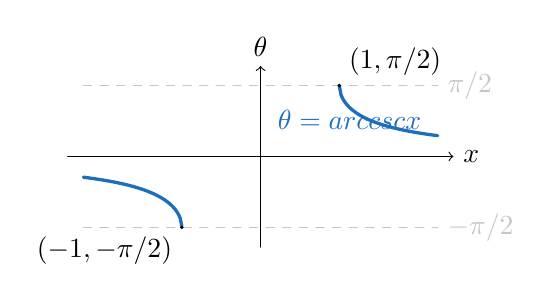
\begin{tikzpicture}[scale=1.0, line cap=round, line join=round]
  \definecolor{trigblue}{RGB}{30,110,190}
  \draw[->] (-2.45,0)--(2.45,0) node[right] {$x$};
  \draw[->] (0,-1.15)--(0,1.15) node[above] {$\theta$};
  \draw[gray!45,dashed] (-2.25,0.9)--(2.25,0.9) node[right] {$\pi/2$};
  \draw[gray!45,dashed] (-2.25,-0.9)--(2.25,-0.9) node[right] {$-\pi/2$};
  \draw[very thick,trigblue,domain=1:2.25,samples=60]
    plot ({\x},{0.9*asin(1/\x)/90});
  \draw[very thick,trigblue,domain=-2.25:-1,samples=60]
    plot ({\x},{0.9*asin(1/\x)/90});
  \fill (1,0.9) circle (0.025) node[above right] {$(1,\pi/2)$};
  \fill (-1,-0.9) circle (0.025) node[below left] {$(-1,-\pi/2)$};
  \node[trigblue] at (1.13,0.47) {$\theta=\operatorname{arccsc} x$};
\end{tikzpicture}
\end{center}


\begin{definitionbox}{Definition}
\begin{definition}[Inverse cosecant]
\label{def:inverse-cosecant}
The \emph{inverse cosecant} function is the inverse of cosecant after cosecant
is restricted to $[-\pi/2,\pi/2]\setminus\{0\}$. It is denoted by $\operatorname{arccsc}$
or $\csc^{-1}$ and has domain $(-\infty,-1]\cup[1,\infty)$ and range
$[-\pi/2,\pi/2]\setminus\{0\}$.
\[
  \operatorname{arccsc} x=\theta
  \quad\Longleftrightarrow\quad
  \csc\theta=x
  \quad\text{and}\quad
  -\frac{\pi}{2}\leq\theta\leq\frac{\pi}{2},\ \theta\neq 0.
\]
\end{definition}
\end{definitionbox}
\begin{remark*}[Standard quantified statement]
For every admissible input satisfying the hypotheses of the statement, the
displayed definition or assertion holds in the stated domain.
\end{remark*}

\begin{remark*}[Interpretation]
The statement records the named trigonometric object or identity together with
its intended domain of use.
\end{remark*}

\begin{remark*}[Domain and range]
The cosecant function has domain
$\mathbb{R}\setminus\{k\pi:k\in\mathbb{Z}\}$ and range
$(-\infty,-1]\cup[1,\infty)$. The inverse cosecant function reverses the
principal restricted cosecant function.
\end{remark*}
\begin{dependencies}
\begin{itemize}
  \item \hyperref[def:extended-cosecant]{Extended cosecant}
  \item \hyperref[def:radian-measure]{Radian measure}
\end{itemize}
\end{dependencies}

\begin{theorembox}{Theorem}
\begin{theorem}[Principal inverse cosecant identities]
\label{thm:inverse-cosecant-identities}
For every $x\in(-\infty,-1]\cup[1,\infty)$,
\[
  \csc(\operatorname{arccsc} x)=x.
\]
For every $\theta\in[-\pi/2,\pi/2]\setminus\{0\}$,
\[
  \operatorname{arccsc}(\csc\theta)=\theta.
\]
\end{theorem}
\end{theorembox}
\begin{remark*}[Interpretation]
The statement records the named trigonometric object or identity together with
its intended domain of use.
\end{remark*}

\begin{remark*}[Standard quantified statement]
$\forall x\in(-\infty,-1]\cup[1,\infty)$, $\csc(\operatorname{arccsc} x)=x$, and
$\forall \theta\in[-\pi/2,\pi/2]\setminus\{0\}$,
$\operatorname{arccsc}(\csc\theta)=\theta$.
\end{remark*}
\begin{dependencies}
\begin{itemize}
  \item \hyperref[def:inverse-cosecant]{Inverse cosecant}
\end{itemize}
\end{dependencies}

\begin{theorembox}{Theorem}
\begin{theorem}[Cofunction identities for inverse sine and inverse cosine]
\label{thm:inverse-trig-cofunction-identities}
For every $x\in[-1,1]$,
\[
  \arcsin x+\arccos x=\frac{\pi}{2}.
\]
Equivalently,
\[
  \arccos x=\frac{\pi}{2}-\arcsin x,
  \qquad
  \arcsin x=\frac{\pi}{2}-\arccos x.
\]
\end{theorem}
\end{theorembox}
\begin{remark*}[Standard quantified statement]
$\forall x\in[-1,1]$, $\arcsin x+\arccos x=\pi/2$.
\end{remark*}
\begin{dependencies}
\begin{itemize}
  \item \hyperref[def:inverse-sine]{Inverse sine}
  \item \hyperref[def:inverse-cosine]{Inverse cosine}
\end{itemize}
\end{dependencies}

\begin{theorembox}{Theorem}
\begin{theorem}[Reciprocal identities for inverse secant and inverse cosecant]
\label{thm:inverse-trig-reciprocal-identities}
For every $x\in(-\infty,-1]\cup[1,\infty)$,
\[
  \operatorname{arcsec} x=\arccos\!\left(\frac{1}{x}\right),
  \qquad
  \operatorname{arccsc} x=\arcsin\!\left(\frac{1}{x}\right).
\]
\end{theorem}
\end{theorembox}
\begin{remark*}[Standard quantified statement]
\[
  \forall x\in(-\infty,-1]\cup[1,\infty),\quad
  \operatorname{arcsec} x=\arccos(1/x)
  \quad\text{and}\quad
  \operatorname{arccsc} x=\arcsin(1/x).
\]
\end{remark*}
\begin{dependencies}
\begin{itemize}
  \item \hyperref[def:inverse-cosine]{Inverse cosine}
  \item \hyperref[def:inverse-sine]{Inverse sine}
  \item \hyperref[def:inverse-secant]{Inverse secant}
  \item \hyperref[def:inverse-cosecant]{Inverse cosecant}
\end{itemize}
\end{dependencies}

\begin{theorembox}{Theorem}
\begin{theorem}[Reciprocal identity for inverse cotangent]
\label{thm:inverse-cotangent-reciprocal-identity}
For every nonzero real number $x$,
\[
  \operatorname{arccot} x=
  \begin{cases}
    \arctan(1/x), & x>0,\\
    \pi+\arctan(1/x), & x<0.
  \end{cases}
\]
\end{theorem}
\end{theorembox}
\begin{remark*}[Branch convention]
The second case is necessary because this chapter uses the principal range
$(0,\pi)$ for $\operatorname{arccot}$ and $(-\pi/2,\pi/2)$ for $\arctan$.
\end{remark*}
\begin{dependencies}
\begin{itemize}
  \item \hyperref[def:inverse-tangent]{Inverse tangent}
  \item \hyperref[def:inverse-cotangent]{Inverse cotangent}
\end{itemize}
\end{dependencies}

\begin{remark*}[Standard quantified statement]
For every right triangle $T$ and every acute angle $\theta$ of $T$, the six
displayed ratios are defined whenever the denominator in the displayed quotient
is nonzero.
\end{remark*}

\begin{remark*}[Standard quantified statement]
For every acute Euclidean angle $\theta$, if $T$ is a right triangle having
$\theta$ as an acute angle, then $\sin\theta$ and $\cos\theta$ are the
opposite-over-hypotenuse and adjacent-over-hypotenuse ratios of $T$.
\end{remark*}
\begin{remark*}[Well-definedness debt]
These definitions depend on the similarity-invariance theorem below. Until that
theorem is invoked, the displayed formulas describe a ratio in a chosen
triangle, not yet a function of $\theta$ alone.
\end{remark*}
\begin{dependencies}
\begin{itemize}
  \item \hyperref[def:right-triangle-sine]{Right-triangle sine}
  \item \hyperref[def:right-triangle-cosine]{Right-triangle cosine}
\end{itemize}
\end{dependencies}

\begin{center}
\begin{tikzpicture}[scale=0.95, line cap=round, line join=round]
  \definecolor{trigblue}{RGB}{30,110,190}
  \coordinate (A) at (0,0);
  \coordinate (B) at (2.2,0);
  \coordinate (C) at (2.2,1.25);
  \coordinate (D) at (4.2,0);
  \coordinate (E) at (7.5,0);
  \coordinate (F) at (7.5,1.875);
  \draw[very thick] (A)--(B)--(C)--cycle;
  \draw[very thick] (D)--(E)--(F)--cycle;
  \draw (1.95,0)--(1.95,0.25)--(2.2,0.25);
  \draw (7.2,0)--(7.2,0.3)--(7.5,0.3);
  \draw[trigblue] ($(A)+(0.42,0)$) arc[start angle=0,end angle=29.6,radius=0.42];
  \draw[trigblue] ($(D)+(0.50,0)$) arc[start angle=0,end angle=29.6,radius=0.50];
  \node[trigblue] at (0.55,0.17) {$\theta$};
  \node[trigblue] at (4.85,0.20) {$\theta$};
  \node[font=\footnotesize] at (1.25,-0.35) {$T_1$};
  \node[font=\footnotesize] at (5.95,-0.35) {$T_2$};
  \node[font=\footnotesize] at (3.75,1.2) {same angle, same ratios};
\end{tikzpicture}
\end{center}


\begin{theorembox}{Theorem}
\begin{theorem}[Similarity invariance of trigonometric ratios]
\label{thm:trig-ratios-similarity-invariant}
If two right triangles have the same acute angle $\theta$, then their
corresponding opposite-to-hypotenuse and adjacent-to-hypotenuse ratios are
equal.
\end{theorem}
\end{theorembox}
\begin{remark*}[Interpretation]
The statement records the named trigonometric object or identity together with
its intended domain of use.
\end{remark*}

\begin{remark*}[Proof]
\hyperref[prf:trig-ratios-similarity-invariant]{Go to proof.}
\end{remark*}
\begin{remark*}[Standard quantified statement]
For all right triangles $T_1,T_2$ and every acute angle $\theta$, if $\theta$
is an acute angle of both triangles, then
\[
\frac{\operatorname{opp}(T_1,\theta)}{\operatorname{hyp}(T_1)}
=
\frac{\operatorname{opp}(T_2,\theta)}{\operatorname{hyp}(T_2)}
\quad\text{and}\quad
\frac{\operatorname{adj}(T_1,\theta)}{\operatorname{hyp}(T_1)}
=
\frac{\operatorname{adj}(T_2,\theta)}{\operatorname{hyp}(T_2)}.
\]
\end{remark*}
\begin{dependencies}
\begin{itemize}
  \item \hyperref[thm:euclid-i-32]{Euclid I.32}
\end{itemize}
\end{dependencies}

\begin{center}
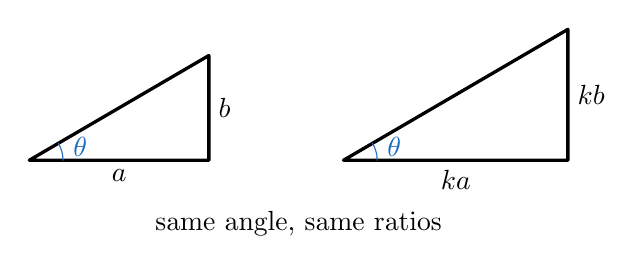
\begin{tikzpicture}[scale=0.95, line cap=round, line join=round]
  \definecolor{trigblue}{RGB}{30,110,190}
  \coordinate (A) at (0,0);
  \coordinate (B) at (2.4,0);
  \coordinate (C) at (2.4,1.4);
  \coordinate (D) at (4.2,0);
  \coordinate (E) at (7.2,0);
  \coordinate (F) at (7.2,1.75);
  \draw[very thick] (A)--(B)--(C)--cycle;
  \draw[very thick] (D)--(E)--(F)--cycle;
  \draw[trigblue] (0.45,0) arc[start angle=0,end angle=30.3,radius=0.45];
  \draw[trigblue] (4.65,0) arc[start angle=0,end angle=30.3,radius=0.45];
  \node[trigblue] at (0.68,0.18) {$\theta$};
  \node[trigblue] at (4.88,0.18) {$\theta$};
  \node[below] at (1.2,0) {$a$};
  \node[right] at (2.4,0.7) {$b$};
  \node[below] at (5.7,0) {$ka$};
  \node[right] at (7.2,0.88) {$kb$};
  \node[below] at (3.6,-0.55) {same angle, same ratios};
\end{tikzpicture}
\end{center}


\begin{theorembox}{Theorem}
\begin{theorem}[Well-definedness of sine and cosine]
\label{thm:sine-cosine-well-defined}
For each acute Euclidean angle $\theta$, the values $\sin\theta$ and
\(\cos\theta\) are independent of the right triangle chosen to compute them.
\end{theorem}
\end{theorembox}
\begin{remark*}[Standard quantified statement]
For every admissible input satisfying the hypotheses of the statement, the
displayed definition or assertion holds in the stated domain.
\end{remark*}

\begin{remark*}[Interpretation]
The statement records the named trigonometric object or identity together with
its intended domain of use.
\end{remark*}

\begin{remark*}[Proof]
\hyperref[prf:sine-cosine-well-defined]{Go to proof.}
\end{remark*}
\begin{dependencies}
\begin{itemize}
  \item \hyperref[def:acute-angle-sine]{Acute-angle sine}
  \item \hyperref[def:acute-angle-cosine]{Acute-angle cosine}
  \item \hyperref[thm:trig-ratios-similarity-invariant]{Similarity invariance of trigonometric ratios}
\end{itemize}
\end{dependencies}

\begin{center}
\begin{tikzpicture}[scale=1.05, line cap=round, line join=round]
  \definecolor{trigblue}{RGB}{30,110,190}
  \coordinate (A) at (0,0);
  \coordinate (B) at (3.2,0);
  \coordinate (C) at (3.2,1.85);
  \draw[very thick] (A)--(B)--(C)--cycle;
  \draw (2.9,0)--(2.9,0.3)--(3.2,0.3);
  \draw[trigblue] (0.5,0) arc[start angle=0,end angle=30,radius=0.5];
  \node[trigblue] at (0.72,0.2) {$\theta$};
  \node[below] at ($(A)!0.5!(B)$) {$a$};
  \node[right] at ($(B)!0.5!(C)$) {$o$};
  \node[above left] at ($(A)!0.5!(C)$) {$h$};
  \node[right] at (4.0,1.45) {$\sin=o/h,\quad \cos=a/h$};
  \node[right] at (4.0,0.95) {$\tan=o/a,\quad \cot=a/o$};
  \node[right] at (4.0,0.45) {$\sec=h/a,\quad \csc=h/o$};
\end{tikzpicture}
\end{center}


\begin{theorembox}{Theorem}
\begin{theorem}[Six trigonometric functions]
\label{thm:six-trig-functions}
The six right-triangle trigonometric ratios define functions of an acute
Euclidean angle, subject to the denominator restrictions in their defining
quotients.
\end{theorem}
\end{theorembox}
\begin{remark*}[Standard quantified statement]
For every admissible input satisfying the hypotheses of the statement, the
displayed definition or assertion holds in the stated domain.
\end{remark*}

\begin{remark*}[Interpretation]
The statement records the named trigonometric object or identity together with
its intended domain of use.
\end{remark*}

\begin{remark*}[Proof]
\hyperref[prf:six-trig-functions]{Go to proof.}
\end{remark*}
\begin{dependencies}
\begin{itemize}
  \item \hyperref[def:right-triangle-sine]{Right-triangle sine}
  \item \hyperref[def:right-triangle-cosine]{Right-triangle cosine}
  \item \hyperref[thm:sine-cosine-well-defined]{Well-definedness of sine and cosine}
\end{itemize}
\end{dependencies}

\begin{remark*}[Debt flag]
This definition extends sine and cosine beyond acute angles. Treating
$\theta$ as an arbitrary real-valued radian input requires arc length and
rectifiability machinery not yet developed in this volume.
\end{remark*}
\begin{dependencies}
\begin{itemize}
  \item \hyperref[def:euclid-circle]{Circle}
  \item \hyperref[def:cartesian-product]{Cartesian Product}
  \item \hyperref[thm:sine-cosine-well-defined]{Well-definedness of sine and cosine}
\end{itemize}
\end{dependencies}

\begin{center}
\begin{tikzpicture}[scale=1.45, line cap=round, line join=round]
  \definecolor{trigblue}{RGB}{30,110,190}
  \coordinate (O) at (0,0);
  \coordinate (P) at (32:1);
  \coordinate (Q) at ({cos(32)},0);
  \draw[gray!55] (O) circle (1);
  \draw[->] (-0.15,0)--(1.3,0) node[right] {$x$};
  \draw[->] (0,-0.15)--(0,1.15) node[above] {$y$};
  \draw[very thick] (O)--(Q)--(P)--cycle;
  \draw[trigblue] (0.3,0) arc[start angle=0,end angle=32,radius=0.3];
  \node[trigblue] at (0.35,0.1) {$\theta$};
  \node[below] at ($(O)!0.5!(Q)$) {$\cos\theta$};
  \node[right] at ($(Q)!0.5!(P)$) {$\sin\theta$};
  \node[above left] at ($(O)!0.5!(P)$) {$1$};
\end{tikzpicture}
\end{center}


\begin{theorembox}{Theorem}
\begin{theorem}[Unit-circle agreement with right-triangle trigonometry]
\label{thm:unit-circle-agrees-with-right-triangle-trig}
For $0<\theta<90^\circ$, the unit-circle definitions of sine and cosine agree
with the right-triangle definitions.
\end{theorem}
\end{theorembox}
\begin{remark*}[Standard quantified statement]
For every admissible input satisfying the hypotheses of the statement, the
displayed definition or assertion holds in the stated domain.
\end{remark*}

\begin{remark*}[Interpretation]
The statement records the named trigonometric object or identity together with
its intended domain of use.
\end{remark*}

\begin{remark*}[Proof]
\hyperref[prf:unit-circle-agrees-with-right-triangle-trig]{Go to proof.}
\end{remark*}
\begin{dependencies}
\begin{itemize}
  \item \hyperref[def:acute-angle-sine]{Acute-angle sine}
  \item \hyperref[def:acute-angle-cosine]{Acute-angle cosine}
  \item \hyperref[def:unit-circle-cosine]{Unit-circle cosine}
  \item \hyperref[def:unit-circle-sine]{Unit-circle sine}
\end{itemize}
\end{dependencies}

\begin{dependencies}
\begin{itemize}
  \item \hyperref[def:unit-circle-cosine]{Unit-circle cosine}
  \item \hyperref[def:unit-circle-sine]{Unit-circle sine}
  \item \hyperref[thm:unit-circle-agrees-with-right-triangle-trig]{Unit-circle agreement with right-triangle trigonometry}
\end{itemize}
\end{dependencies}

\begin{center}
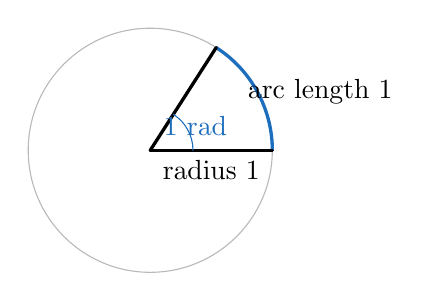
\begin{tikzpicture}[scale=1.55, line cap=round, line join=round]
  \definecolor{trigblue}{RGB}{30,110,190}
  \coordinate (O) at (0,0);
  \draw[gray!55] (O) circle (1);
  \draw[very thick,trigblue] (1,0) arc[start angle=0,end angle=57.3,radius=1];
  \draw[very thick] (O)--(1,0);
  \draw[very thick] (O)--(57.3:1);
  \draw[trigblue] (0.35,0) arc[start angle=0,end angle=57.3,radius=0.35];
  \node[trigblue] at (0.37,0.2) {$1$ rad};
  \node[right] at (0.72,0.48) {arc length $1$};
  \node[below] at (0.5,0) {radius $1$};
\end{tikzpicture}
\end{center}


\begin{definitionbox}{Definition}
\begin{definition}[Radian measure]
\label{def:radian-measure}
One radian is the angle that cuts off arc length $1$ on the unit circle. A full
turn has measure $2\pi$ radians.
\end{definition}
\end{definitionbox}
\begin{remark*}[Standard quantified statement]
For every admissible input satisfying the hypotheses of the statement, the
displayed definition or assertion holds in the stated domain.
\end{remark*}

\begin{remark*}[Interpretation]
The statement records the named trigonometric object or identity together with
its intended domain of use.
\end{remark*}

\begin{remark*}[Debt flag]
This definition uses arc length intuitively. Its rigorous foundation belongs
after rectifiable curves and the construction of $\pi$ from circumference.
\end{remark*}
\begin{dependencies}
\begin{itemize}
  \item \hyperref[def:unit-circle-cosine]{Unit-circle cosine}
  \item \hyperref[def:unit-circle-sine]{Unit-circle sine}
  \item \hyperref[def:euclid-circle]{Circle}
\end{itemize}
\end{dependencies}

\begin{center}
\begin{tikzpicture}[scale=1.35, line cap=round, line join=round]
  \definecolor{trigblue}{RGB}{30,110,190}
  \coordinate (O) at (0,0);
  \coordinate (P) at (35:1);
  \coordinate (Q) at (-35:1);
  \draw[gray!55] (O) circle (1);
  \draw[->] (-1.25,0)--(1.35,0) node[right] {$x$};
  \draw[->] (0,-1.15)--(0,1.25) node[above] {$y$};
  \draw[very thick,trigblue] (O)--(P);
  \draw[very thick,trigblue] (O)--(Q);
  \draw[dropline] (P)--({cos(35)},0)--(Q);
  \fill (P) circle (0.02) node[above right] {$\theta$};
  \fill (Q) circle (0.02) node[below right] {$-\theta$};
\end{tikzpicture}
\end{center}


\begin{theorembox}{Theorem}
\begin{theorem}[Symmetry and periodicity of sine and cosine]
\label{thm:trig-symmetry-periodicity}
For every angle in the unit-circle domain,
\[
\cos(-\theta)=\cos\theta,\qquad \sin(-\theta)=-\sin\theta,
\]
and one full turn returns the same sine and cosine values.
\end{theorem}
\end{theorembox}
\begin{remark*}[Standard quantified statement]
For every admissible input satisfying the hypotheses of the statement, the
displayed definition or assertion holds in the stated domain.
\end{remark*}

\begin{remark*}[Interpretation]
The statement records the named trigonometric object or identity together with
its intended domain of use.
\end{remark*}

\begin{remark*}[Proof]
\hyperref[prf:trig-symmetry-periodicity]{Go to proof.}
\end{remark*}
\begin{dependencies}
\begin{itemize}
  \item \hyperref[def:unit-circle-cosine]{Unit-circle cosine}
  \item \hyperref[def:unit-circle-sine]{Unit-circle sine}
  \item \hyperref[def:radian-measure]{Radian measure}
\end{itemize}
\end{dependencies}

\input{volume-i/book-geometry/trigonometry/foundations/figure-pythagorean-trig-identity}

\begin{theorembox}{Theorem}
\begin{theorem}[Pythagorean identity]
\label{thm:pythagorean-trig-identity}
For every angle in the unit-circle domain,
\[
  \cos^2\theta+\sin^2\theta=1.
\]
\end{theorem}
\end{theorembox}
\begin{remark*}[Standard quantified statement]
For every admissible input satisfying the hypotheses of the statement, the
displayed definition or assertion holds in the stated domain.
\end{remark*}

\begin{remark*}[Interpretation]
The statement records the named trigonometric object or identity together with
its intended domain of use.
\end{remark*}

\begin{remark*}[Proof]
\hyperref[prf:pythagorean-trig-identity]{Go to proof.}
\end{remark*}
\begin{dependencies}
\begin{itemize}
  \item \hyperref[thm:euclid-i-47]{Euclid I.47}
  \item \hyperref[def:unit-circle-cosine]{Unit-circle cosine}
  \item \hyperref[def:unit-circle-sine]{Unit-circle sine}
\end{itemize}
\end{dependencies}

\begin{center}
\begin{tikzpicture}[scale=1.3, line cap=round, line join=round]
  \definecolor{trigblue}{RGB}{30,110,190}
  \coordinate (O) at (0,0);
  \coordinate (P) at (36:1);
  \coordinate (T) at (1,{tan(36)});
  \draw[gray!55] (O) circle (1);
  \draw[->] (-0.2,0)--(1.35,0) node[right] {$x$};
  \draw[->] (0,-0.2)--(0,1.25) node[above] {$y$};
  \draw[gray!70] (1,-0.1)--(1,1.2);
  \draw[very thick] (O)--(P);
  \draw[very thick,trigblue] (O)--(T);
  \fill (P) circle (0.02) node[above left] {$\cos\theta,\sin\theta$};
  \node[above left,trigblue] at ($(O)!0.55!(T)$) {$\sec\theta=1/\cos\theta$};
\end{tikzpicture}
\end{center}


\begin{theorembox}{Theorem}
\begin{theorem}[Reciprocal identities]
\label{thm:trig-reciprocal-identities}
Where both sides are defined,
\[
  \sec\theta=\frac{1}{\cos\theta},\qquad
  \csc\theta=\frac{1}{\sin\theta},\qquad
  \cot\theta=\frac{1}{\tan\theta}.
\]
\end{theorem}
\end{theorembox}
\begin{remark*}[Standard quantified statement]
For every admissible input satisfying the hypotheses of the statement, the
displayed definition or assertion holds in the stated domain.
\end{remark*}

\begin{remark*}[Interpretation]
The statement records the named trigonometric object or identity together with
its intended domain of use.
\end{remark*}

\begin{remark*}[Proof]
\hyperref[prf:trig-reciprocal-identities]{Go to proof.}
\end{remark*}
\begin{dependencies}
\begin{itemize}
  \item \hyperref[def:extended-tangent]{Extended tangent}
  \item \hyperref[def:extended-cotangent]{Extended cotangent}
  \item \hyperref[def:extended-secant]{Extended secant}
  \item \hyperref[def:extended-cosecant]{Extended cosecant}
\end{itemize}
\end{dependencies}

\begin{center}
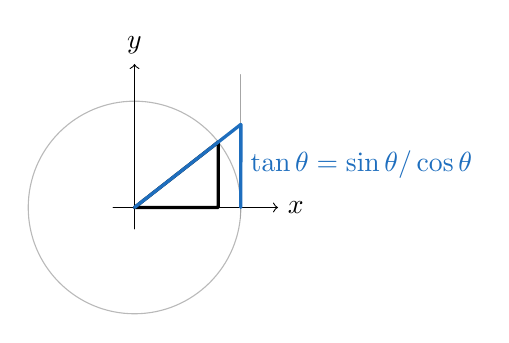
\begin{tikzpicture}[scale=1.35, line cap=round, line join=round]
  \definecolor{trigblue}{RGB}{30,110,190}
  \coordinate (O) at (0,0);
  \coordinate (P) at (38:1);
  \coordinate (Q) at ({cos(38)},0);
  \coordinate (T) at (1,{tan(38)});
  \draw[gray!55] (O) circle (1);
  \draw[->] (-0.2,0)--(1.35,0) node[right] {$x$};
  \draw[->] (0,-0.2)--(0,1.35) node[above] {$y$};
  \draw[gray!70] (1,-0.1)--(1,1.25);
  \draw[very thick] (O)--(Q)--(P)--cycle;
  \draw[very thick,trigblue] (O)--(T);
  \draw[very thick,trigblue] (1,0)--(T);
  \node[right,trigblue] at (1,0.4) {$\tan\theta=\sin\theta/\cos\theta$};
\end{tikzpicture}
\end{center}


\begin{theorembox}{Theorem}
\begin{theorem}[Quotient identities]
\label{thm:trig-quotient-identities}
Where both sides are defined,
\[
  \tan\theta=\frac{\sin\theta}{\cos\theta},\qquad
  \cot\theta=\frac{\cos\theta}{\sin\theta}.
\]
\end{theorem}
\end{theorembox}
\begin{remark*}[Standard quantified statement]
For every admissible input satisfying the hypotheses of the statement, the
displayed definition or assertion holds in the stated domain.
\end{remark*}

\begin{remark*}[Interpretation]
The statement records the named trigonometric object or identity together with
its intended domain of use.
\end{remark*}

\begin{remark*}[Proof]
\hyperref[prf:trig-quotient-identities]{Go to proof.}
\end{remark*}
\begin{dependencies}
\begin{itemize}
  \item \hyperref[def:extended-tangent]{Extended tangent}
  \item \hyperref[def:extended-cotangent]{Extended cotangent}
\end{itemize}
\end{dependencies}

\begin{center}
\begin{tikzpicture}[scale=1.3, line cap=round, line join=round]
  \definecolor{trigblue}{RGB}{30,110,190}
  \coordinate (O) at (0,0);
  \coordinate (T) at (1,{tan(38)});
  \draw[->] (-0.2,0)--(1.35,0) node[right] {$x$};
  \draw[->] (0,-0.2)--(0,1.35) node[above] {$y$};
  \draw[gray!70] (1,-0.1)--(1,1.25);
  \draw[very thick] (O)--(1,0)--(T)--cycle;
  \draw[trigblue] (0.35,0) arc[start angle=0,end angle=38,radius=0.35];
  \node[below] at (0.5,0) {$1$};
  \node[right] at (1,0.4) {$\tan\theta$};
  \node[above left,trigblue] at ($(O)!0.55!(T)$) {$\sec\theta$};
\end{tikzpicture}
\end{center}


\begin{theorembox}{Theorem}
\begin{theorem}[Tangent and secant Pythagorean identities]
\label{thm:trig-tangent-pythagorean-identities}
Where both sides are defined,
\[
  1+\tan^2\theta=\sec^2\theta,
  \qquad
  1+\cot^2\theta=\csc^2\theta.
\]
\end{theorem}
\end{theorembox}
\begin{remark*}[Standard quantified statement]
For every admissible input satisfying the hypotheses of the statement, the
displayed definition or assertion holds in the stated domain.
\end{remark*}

\begin{remark*}[Interpretation]
The statement records the named trigonometric object or identity together with
its intended domain of use.
\end{remark*}

\begin{remark*}[Proof]
\hyperref[prf:trig-tangent-pythagorean-identities]{Go to proof.}
\end{remark*}
\begin{dependencies}
\begin{itemize}
  \item \hyperref[thm:pythagorean-trig-identity]{Pythagorean identity}
  \item \hyperref[thm:trig-quotient-identities]{Quotient identities}
  \item \hyperref[thm:trig-reciprocal-identities]{Reciprocal identities}
\end{itemize}
\end{dependencies}

\begin{center}
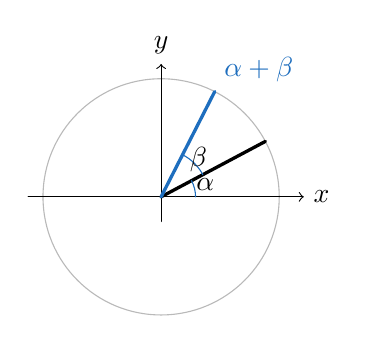
\begin{tikzpicture}[scale=1.25, line cap=round, line join=round]
  \definecolor{trigblue}{RGB}{30,110,190}
  \draw[gray!55] (0,0) circle (1.2);
  \draw[->] (-1.35,0)--(1.45,0) node[right] {$x$};
  \draw[->] (0,-0.25)--(0,1.35) node[above] {$y$};
  \draw[very thick] (0,0)--(28:1.2);
  \draw[very thick,trigblue] (0,0)--(63:1.2);
  \draw[trigblue] (0.35,0) arc[start angle=0,end angle=28,radius=0.35];
  \draw[trigblue] (28:0.48) arc[start angle=28,end angle=63,radius=0.48];
  \node at (0.45,0.13) {$\alpha$};
  \node at (0.38,0.38) {$\beta$};
  \node[above right,trigblue] at (63:1.2) {$\alpha+\beta$};
\end{tikzpicture}
\end{center}


\begin{theorembox}{Theorem}
\begin{theorem}[Angle-sum identities]
\label{thm:trig-angle-sum-identities}
For angles in the unit-circle domain,
\[
  \cos(\alpha+\beta)=\cos\alpha\cos\beta-\sin\alpha\sin\beta,
\]
\[
  \sin(\alpha+\beta)=\sin\alpha\cos\beta+\cos\alpha\sin\beta.
\]
\end{theorem}
\end{theorembox}
\begin{remark*}[Standard quantified statement]
For every admissible input satisfying the hypotheses of the statement, the
displayed definition or assertion holds in the stated domain.
\end{remark*}

\begin{remark*}[Interpretation]
The statement records the named trigonometric object or identity together with
its intended domain of use.
\end{remark*}

\begin{remark*}[Proof]
\hyperref[prf:trig-angle-sum-identities]{Go to proof.}
\end{remark*}
\begin{dependencies}
\begin{itemize}
  \item \hyperref[thm:pythagorean-trig-identity]{Pythagorean identity}
\end{itemize}
\end{dependencies}

\begin{center}
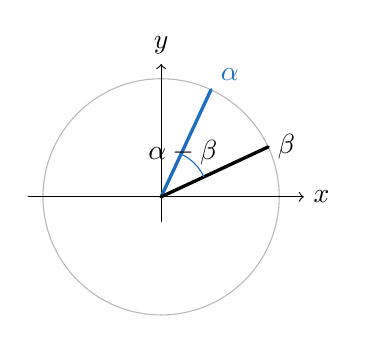
\begin{tikzpicture}[scale=1.25, line cap=round, line join=round]
  \definecolor{trigblue}{RGB}{30,110,190}
  \draw[gray!55] (0,0) circle (1.2);
  \draw[->] (-1.35,0)--(1.45,0) node[right] {$x$};
  \draw[->] (0,-0.25)--(0,1.35) node[above] {$y$};
  \draw[very thick,trigblue] (0,0)--(65:1.2);
  \draw[very thick] (0,0)--(25:1.2);
  \draw[trigblue] (25:0.48) arc[start angle=25,end angle=65,radius=0.48];
  \node at (0.22,0.45) {$\alpha-\beta$};
  \node[above right,trigblue] at (65:1.2) {$\alpha$};
  \node[right] at (25:1.2) {$\beta$};
\end{tikzpicture}
\end{center}


\begin{theorembox}{Theorem}
\begin{theorem}[Angle-difference identities]
\label{thm:trig-angle-difference-identities}
For angles in the unit-circle domain,
\[
  \cos(\alpha-\beta)=\cos\alpha\cos\beta+\sin\alpha\sin\beta,
\]
\[
  \sin(\alpha-\beta)=\sin\alpha\cos\beta-\cos\alpha\sin\beta.
\]
\end{theorem}
\end{theorembox}
\begin{remark*}[Standard quantified statement]
For every admissible input satisfying the hypotheses of the statement, the
displayed definition or assertion holds in the stated domain.
\end{remark*}

\begin{remark*}[Interpretation]
The statement records the named trigonometric object or identity together with
its intended domain of use.
\end{remark*}

\begin{remark*}[Proof]
\hyperref[prf:trig-angle-difference-identities]{Go to proof.}
\end{remark*}
\begin{dependencies}
\begin{itemize}
  \item \hyperref[thm:trig-angle-sum-identities]{Angle-sum identities}
  \item \hyperref[thm:trig-symmetry-periodicity]{Symmetry and periodicity of sine and cosine}
\end{itemize}
\end{dependencies}

\begin{center}
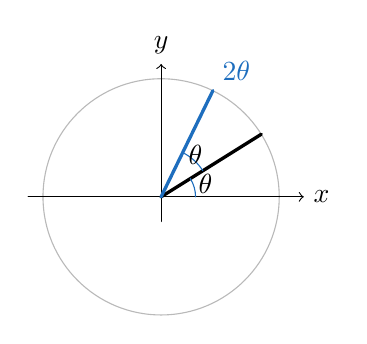
\begin{tikzpicture}[scale=1.25, line cap=round, line join=round]
  \definecolor{trigblue}{RGB}{30,110,190}
  \draw[gray!55] (0,0) circle (1.2);
  \draw[->] (-1.35,0)--(1.45,0) node[right] {$x$};
  \draw[->] (0,-0.25)--(0,1.35) node[above] {$y$};
  \draw[very thick] (0,0)--(32:1.2);
  \draw[very thick,trigblue] (0,0)--(64:1.2);
  \draw[trigblue] (0.35,0) arc[start angle=0,end angle=32,radius=0.35];
  \draw[trigblue] (32:0.5) arc[start angle=32,end angle=64,radius=0.5];
  \node at (0.45,0.13) {$\theta$};
  \node at (0.35,0.43) {$\theta$};
  \node[above right,trigblue] at (64:1.2) {$2\theta$};
\end{tikzpicture}
\end{center}


\begin{theorembox}{Theorem}
\begin{theorem}[Double-angle identities]
\label{thm:trig-double-angle-identities}
For angles in the unit-circle domain,
\[
  \sin(2\theta)=2\sin\theta\cos\theta,
\]
\[
  \cos(2\theta)=\cos^2\theta-\sin^2\theta
  =2\cos^2\theta-1
  =1-2\sin^2\theta.
\]
\end{theorem}
\end{theorembox}
\begin{remark*}[Standard quantified statement]
For every admissible input satisfying the hypotheses of the statement, the
displayed definition or assertion holds in the stated domain.
\end{remark*}

\begin{remark*}[Interpretation]
The statement records the named trigonometric object or identity together with
its intended domain of use.
\end{remark*}

\begin{remark*}[Proof]
\hyperref[prf:trig-double-angle-identities]{Go to proof.}
\end{remark*}
\begin{dependencies}
\begin{itemize}
  \item \hyperref[thm:trig-angle-sum-identities]{Angle-sum identities}
  \item \hyperref[thm:pythagorean-trig-identity]{Pythagorean identity}
\end{itemize}
\end{dependencies}

\begin{center}
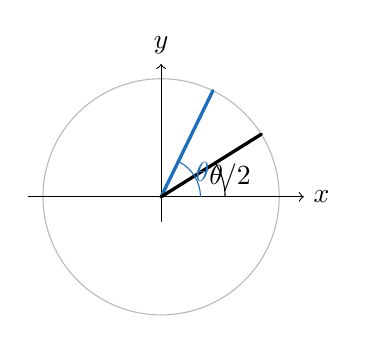
\begin{tikzpicture}[scale=1.25, line cap=round, line join=round]
  \definecolor{trigblue}{RGB}{30,110,190}
  \draw[gray!55] (0,0) circle (1.2);
  \draw[->] (-1.35,0)--(1.45,0) node[right] {$x$};
  \draw[->] (0,-0.25)--(0,1.35) node[above] {$y$};
  \draw[very thick,trigblue] (0,0)--(64:1.2);
  \draw[very thick] (0,0)--(32:1.2);
  \draw[trigblue] (0.4,0) arc[start angle=0,end angle=64,radius=0.4];
  \draw (0.65,0) arc[start angle=0,end angle=32,radius=0.65];
  \node[trigblue] at (0.42,0.25) {$\theta$};
  \node at (0.7,0.2) {$\theta/2$};
\end{tikzpicture}
\end{center}


\begin{theorembox}{Theorem}
\begin{theorem}[Half-angle identities]
\label{thm:trig-half-angle-identities}
Where the signs are chosen according to the quadrant of $\theta/2$,
\[
  \sin\frac{\theta}{2}=\pm\sqrt{\frac{1-\cos\theta}{2}},
  \qquad
  \cos\frac{\theta}{2}=\pm\sqrt{\frac{1+\cos\theta}{2}}.
\]
\end{theorem}
\end{theorembox}
\begin{remark*}[Standard quantified statement]
For every admissible input satisfying the hypotheses of the statement, the
displayed definition or assertion holds in the stated domain.
\end{remark*}

\begin{remark*}[Interpretation]
The statement records the named trigonometric object or identity together with
its intended domain of use.
\end{remark*}

\begin{remark*}[Proof]
\hyperref[prf:trig-half-angle-identities]{Go to proof.}
\end{remark*}
\begin{dependencies}
\begin{itemize}
  \item \hyperref[thm:trig-double-angle-identities]{Double-angle identities}
\end{itemize}
\end{dependencies}

\begin{center}
\begin{tikzpicture}[scale=1.2, line cap=round, line join=round]
  \definecolor{trigblue}{RGB}{30,110,190}
  \draw[gray!55] (0,0) circle (1.2);
  \draw[->] (-1.35,0)--(1.45,0) node[right] {$x$};
  \draw[->] (0,-0.25)--(0,1.35) node[above] {$y$};
  \draw[very thick,trigblue] (0,0)--(65:1.2);
  \draw[very thick] (0,0)--(25:1.2);
  \draw[dropline] (65:1.2)--({1.2*cos(65)},0);
  \draw[dropline] (25:1.2)--({1.2*cos(25)},0);
  \node[above right,trigblue] at (65:1.2) {$\alpha$};
  \node[right] at (25:1.2) {$\beta$};
  \node[below] at (0,-0.35) {products from paired projections};
\end{tikzpicture}
\end{center}


\begin{theorembox}{Theorem}
\begin{theorem}[Product-to-sum identities]
\label{thm:trig-product-to-sum-identities}
For angles in the unit-circle domain,
\[
\sin\alpha\cos\beta
=\frac{\sin(\alpha+\beta)+\sin(\alpha-\beta)}{2},
\]
\[
\cos\alpha\cos\beta
=\frac{\cos(\alpha+\beta)+\cos(\alpha-\beta)}{2},
\]
\[
\sin\alpha\sin\beta
=\frac{\cos(\alpha-\beta)-\cos(\alpha+\beta)}{2}.
\]
\end{theorem}
\end{theorembox}
\begin{remark*}[Standard quantified statement]
For every admissible input satisfying the hypotheses of the statement, the
displayed definition or assertion holds in the stated domain.
\end{remark*}

\begin{remark*}[Interpretation]
The statement records the named trigonometric object or identity together with
its intended domain of use.
\end{remark*}

\begin{remark*}[Proof]
\hyperref[prf:trig-product-to-sum-identities]{Go to proof.}
\end{remark*}
\begin{dependencies}
\begin{itemize}
  \item \hyperref[thm:trig-angle-sum-identities]{Angle-sum identities}
  \item \hyperref[thm:trig-angle-difference-identities]{Angle-difference identities}
\end{itemize}
\end{dependencies}

\begin{center}
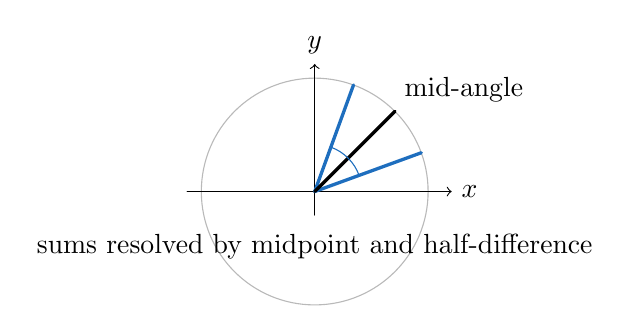
\begin{tikzpicture}[scale=1.2, line cap=round, line join=round]
  \definecolor{trigblue}{RGB}{30,110,190}
  \draw[gray!55] (0,0) circle (1.2);
  \draw[->] (-1.35,0)--(1.45,0) node[right] {$x$};
  \draw[->] (0,-0.25)--(0,1.35) node[above] {$y$};
  \draw[very thick,trigblue] (0,0)--(70:1.2);
  \draw[very thick,trigblue] (0,0)--(20:1.2);
  \draw[very thick] (0,0)--(45:1.2);
  \draw[trigblue] (20:0.5) arc[start angle=20,end angle=70,radius=0.5];
  \node[above right] at (45:1.2) {mid-angle};
  \node[below] at (0,-0.35) {sums resolved by midpoint and half-difference};
\end{tikzpicture}
\end{center}


\begin{theorembox}{Theorem}
\begin{theorem}[Sum-to-product identities]
\label{thm:trig-sum-to-product-identities}
For angles in the unit-circle domain,
\[
\sin u+\sin v
=2\sin\frac{u+v}{2}\cos\frac{u-v}{2},
\]
\[
\cos u+\cos v
=2\cos\frac{u+v}{2}\cos\frac{u-v}{2},
\]
\[
\cos u-\cos v
=-2\sin\frac{u+v}{2}\sin\frac{u-v}{2}.
\]
\end{theorem}
\end{theorembox}
\begin{remark*}[Standard quantified statement]
For every admissible input satisfying the hypotheses of the statement, the
displayed definition or assertion holds in the stated domain.
\end{remark*}

\begin{remark*}[Interpretation]
The statement records the named trigonometric object or identity together with
its intended domain of use.
\end{remark*}

\begin{remark*}[Proof]
\hyperref[prf:trig-sum-to-product-identities]{Go to proof.}
\end{remark*}
\begin{dependencies}
\begin{itemize}
  \item \hyperref[thm:trig-product-to-sum-identities]{Product-to-sum identities}
\end{itemize}
\end{dependencies}

\begin{center}
\begin{tikzpicture}[scale=1.05, line cap=round, line join=round]
  \coordinate (A) at (0,0);
  \coordinate (B) at (1.8,0);
  \coordinate (C) at (1.8,1.8);
  \coordinate (D) at (4.0,0);
  \coordinate (E) at (6.4,0);
  \coordinate (F) at (6.4,{2.4*sqrt(3)});
  \draw[very thick] (A)--(B)--(C)--cycle;
  \draw[very thick] (D)--(E)--(F)--cycle;
  \draw (1.55,0)--(1.55,0.25)--(1.8,0.25);
  \draw (6.1,0)--(6.1,0.3)--(6.4,0.3);
  \node[below] at ($(A)!0.5!(B)$) {$1$};
  \node[right] at ($(B)!0.5!(C)$) {$1$};
  \node[above left] at ($(A)!0.5!(C)$) {$\sqrt2$};
  \node[below] at ($(D)!0.5!(E)$) {$1$};
  \node[right] at ($(E)!0.5!(F)$) {$\sqrt3$};
  \node[above left] at ($(D)!0.5!(F)$) {$2$};
  \node at (0.55,0.18) {$45^\circ$};
  \node at (4.56,0.18) {$60^\circ$};
  \node at (6.05,0.58) {$30^\circ$};
\end{tikzpicture}
\end{center}


\begin{remark*}[Special angles]
The $45^\circ$ and $30^\circ$--$60^\circ$ values come from the isosceles right
triangle and the bisected equilateral triangle. The radian entries use the
radian convention above and inherit its arc-length debt.
\end{remark*}

\subsection{Hyperbolic Trigonometric Functions from Geometry}

\begin{remark*}[Motivating picture]
Circular trigonometry reads coordinates from the unit circle
$x^2+y^2=1$. Hyperbolic trigonometry uses the same geometric idea with the
unit rectangular hyperbola
\[
  x^2-y^2=1
\]
in place of the circle. The parameter is not an angle. It is twice the signed
area of the hyperbolic sector swept from the vertex $(1,0)$ to the point on
the right branch.
\end{remark*}

\begin{center}
\input{volume-i/book-geometry/trigonometry/foundations/hyperbolic/figure-atlas-fallback}
\begin{tikzpicture}[scale=1.45, line cap=round, line join=round]
  \draw[atlas axes] (-0.25,0)--(3.25,0) node[right] {$x$};
  \draw[atlas axes] (0,-0.25)--(0,2.35) node[above] {$y$};

  \fill[atlasgold!20]
    (0,0)--(1,0)
    -- plot[domain=1:2.35,samples=90,smooth] (\x,{sqrt(\x*\x-1)})
    -- cycle;
  \draw[atlasgray!65, line width=0.7pt] (0,0)--(2.35,{sqrt(2.35*2.35-1)});
  \draw[atlasgray!65, line width=0.7pt] (0,0)--(1,0);
  \draw[atlasblue, atlas curve]
    plot[domain=1:3.05,samples=120,smooth] (\x,{sqrt(\x*\x-1)});
  \draw[atlasblue, atlas curve]
    plot[domain=1:3.05,samples=120,smooth] (\x,{-sqrt(\x*\x-1)});

  \coordinate (V) at (1,0);
  \coordinate (P) at (2.35,{sqrt(2.35*2.35-1)});
  \fill[atlas dot] (V) node[below] {$V=(1,0)$};
  \fill[atlas dot] (P) node[above left] {$P_t=(\cosh t,\sinh t)$};
  \draw[dropline] (P)--(2.35,0) node[below] {$\cosh t$};
  \draw[dropline] (P)--(0,{sqrt(2.35*2.35-1)}) node[left] {$\sinh t$};
  \node[atlasgold!70!black] at (1.24,0.48) {$t/2$};
  \node[atlasblue] at (2.6,1.65) {$x^2-y^2=1$};
\end{tikzpicture}

\atlascaption{H1}{Hyperbolic sector}{The parameter $t$ is twice the shaded sector area.}
\end{center}


\begin{remark*}[Construction versus behavior]
This chapter gives the geometric construction. Continuity and differentiation
statements are recorded below as forward pointers to the later analysis
chapter on the behavior of elementary functions, where limits, continuity, and
differentiation provide the canonical proofs.
\end{remark*}
\begin{dependencies}
\begin{itemize}
  \item \hyperref[def:cartesian-product]{Cartesian Product}
  \item \hyperref[def:radian-measure]{Radian measure}
\end{itemize}
\end{dependencies}

\begin{definitionbox}{Definition}
\begin{definition}[Hyperbolic sector]
\label{def:hyperbolic-sector}
Let $O=(0,0)$ and $V=(1,0)$. For a point $P=(u,v)$ on the right branch of
$x^2-y^2=1$, write
\[
  \operatorname{HArea}(O,V,P)
\]
for the signed area of the region bounded by the segment $OV$, the segment
$OP$, and the hyperbolic arc from $V$ to $P$. The sign is positive on the
upper branch and negative on the lower branch.
\end{definition}
\end{definitionbox}
\begin{remark*}[Predicate form]
\[
  \operatorname{Sector}(P,t)
  \;\Longleftrightarrow\;
  P=(u,v),\ u^2-v^2=1,\ u>0,\ \text{and}
  2\operatorname{HArea}(O,V,P)=t.
\]
\end{remark*}
\begin{dependencies}
\begin{itemize}
  \item \hyperref[def:cartesian-product]{Cartesian Product}
\end{itemize}
\end{dependencies}

\begin{definitionbox}{Definition}
\begin{definition}[Swept hyperbola point]
\label{def:swept-hyperbola-point}
For $t\geq 0$, let $P_t$ be the unique point on the upper right branch of
$x^2-y^2=1$ satisfying
\[
  2\operatorname{HArea}(O,V,P_t)=t.
\]
For $t<0$, let $P_t$ be the reflection of $P_{-t}$ across the $x$-axis.
\end{definition}
\end{definitionbox}
\begin{remark*}[Coordinate notation]
The separate hyperbolic sine and cosine definitions below name the two
coordinates of this same point. They are not independent constructions.
\end{remark*}
\begin{dependencies}
\begin{itemize}
  \item \hyperref[def:hyperbolic-sector]{Hyperbolic sector}
\end{itemize}
\end{dependencies}

\begin{center}
\input{volume-i/book-geometry/trigonometry/foundations/hyperbolic/figure-atlas-fallback}
\begin{tikzpicture}[scale=0.82, line cap=round, line join=round]
  \draw[atlas axes] (-3.4,0)--(3.4,0) node[right] {$t$};
  \draw[atlas axes] (0,-3.2)--(0,3.2) node[above] {$y$};
  \draw[dropline] (-3,-3)--(3,3);
  \glowstroke{atlasblue}{-2.35:2.35}{0.5*(exp(\x)-exp(-\x))}
  \node[atlasblue] at (1.65,2.35) {$y=\sinh t$};
  \fill[atlas dot] (0,0) node[below right] {$0$};
\end{tikzpicture}

\atlascaption{H2}{Hyperbolic sine}{Odd, strictly increasing, and unbounded in both directions.}
\end{center}


\begin{definitionbox}{Definition}
\begin{definition}[Hyperbolic sine]
\label{def:hyperbolic-sine}
For each $t\in\mathbb{R}$, define $\sinh t$ to be the second coordinate of
the swept hyperbola point $P_t$:
\[
  P_t=(u,\sinh t).
\]
\end{definition}
\end{definitionbox}
\begin{remark*}[Domain and range]
The function $\sinh:\mathbb{R}\to\mathbb{R}$ has domain all real numbers and
range $\mathbb{R}$. It is odd by reflection of the swept point across the
$x$-axis.
\end{remark*}
\begin{dependencies}
\begin{itemize}
  \item \hyperref[def:swept-hyperbola-point]{Swept hyperbola point}
\end{itemize}
\end{dependencies}

\begin{center}
\input{volume-i/book-geometry/trigonometry/foundations/hyperbolic/figure-atlas-fallback}
\begin{tikzpicture}[scale=0.86, line cap=round, line join=round]
  \draw[atlas axes] (-3.25,0)--(3.25,0) node[right] {$t$};
  \draw[atlas axes] (0,-0.25)--(0,3.35) node[above] {$y$};
  \draw[dropline] (-3,1)--(3,1);
  \glowstroke{atlasgreen}{-2.35:2.35}{0.5*(exp(\x)+exp(-\x))}
  \node[atlasgreen!70!black] at (1.55,2.55) {$y=\cosh t$};
  \fill[atlas dot] (0,1) node[below right] {$(0,1)$};
\end{tikzpicture}

\atlascaption{H3}{Hyperbolic cosine}{Even, with global minimum $1$ at $t=0$.}
\end{center}


\begin{definitionbox}{Definition}
\begin{definition}[Hyperbolic cosine]
\label{def:hyperbolic-cosine}
For each $t\in\mathbb{R}$, define $\cosh t$ to be the first coordinate of
the swept hyperbola point $P_t$:
\[
  P_t=(\cosh t,v).
\]
\end{definition}
\end{definitionbox}
\begin{remark*}[Standard quantified statement]
For every admissible input satisfying the hypotheses of the statement, the
displayed definition or assertion holds in the stated domain.
\end{remark*}

\begin{remark*}[Interpretation]
The statement records the named trigonometric object or identity together with
its intended domain of use.
\end{remark*}

\begin{remark*}[Domain and range]
The function $\cosh:\mathbb{R}\to\mathbb{R}$ has domain all real numbers and
range $[1,\infty)$. It is even by reflection of the swept point across the
$x$-axis.
\end{remark*}
\begin{dependencies}
\begin{itemize}
  \item \hyperref[def:swept-hyperbola-point]{Swept hyperbola point}
\end{itemize}
\end{dependencies}

\begin{center}
\input{volume-i/book-geometry/trigonometry/foundations/hyperbolic/figure-atlas-fallback}
\begin{tikzpicture}[scale=1.0, line cap=round, line join=round]
  \draw[atlas axes] (-3.3,0)--(3.3,0) node[right] {$t$};
  \draw[atlas axes] (0,-1.45)--(0,1.45) node[above] {$y$};
  \draw[dropline] (-3.1,1)--(3.1,1) node[right] {$1$};
  \draw[dropline] (-3.1,-1)--(3.1,-1) node[right] {$-1$};
  \glowstroke{atlasred}{-3:3}{(exp(\x)-exp(-\x))/(exp(\x)+exp(-\x))}
  \node[atlasred] at (1.25,0.58) {$y=\tanh t$};
\end{tikzpicture}

\atlascaption{H4}{Hyperbolic tangent}{Odd, increasing, with horizontal asymptotes $y=\pm 1$.}
\end{center}


\begin{definitionbox}{Definition}
\begin{definition}[Hyperbolic tangent]
\label{def:hyperbolic-tangent}
For each $t\in\mathbb{R}$, define the \emph{hyperbolic tangent} by
\[
  \tanh t=\frac{\sinh t}{\cosh t}.
\]
\end{definition}
\end{definitionbox}
\begin{remark*}[Domain and range]
The function $\tanh$ is defined on all of $\mathbb{R}$ because
$\cosh t\geq 1$. Its range is $(-1,1)$.
\end{remark*}
\begin{dependencies}
\begin{itemize}
  \item \hyperref[def:hyperbolic-sine]{Hyperbolic sine}
  \item \hyperref[def:hyperbolic-cosine]{Hyperbolic cosine}
\end{itemize}
\end{dependencies}

\begin{center}
\input{volume-i/book-geometry/trigonometry/foundations/hyperbolic/figure-atlas-fallback}
\begin{tikzpicture}[scale=0.95, line cap=round, line join=round]
  \draw[atlas axes] (-3.25,0)--(3.25,0) node[right] {$t$};
  \draw[atlas axes] (0,-2.6)--(0,2.6) node[above] {$y$};
  \draw[dropline] (-3.05,1)--(3.05,1) node[right] {$1$};
  \draw[dropline] (-3.05,-1)--(3.05,-1) node[right] {$-1$};
  \draw[dropline] (0,-2.45)--(0,2.45);
  \glowstroke{atlasgold}{0.35:3}{(exp(\x)+exp(-\x))/(exp(\x)-exp(-\x))}
  \glowstroke{atlasgold}{-3:-0.35}{(exp(\x)+exp(-\x))/(exp(\x)-exp(-\x))}
  \node[atlasgold!70!black] at (1.25,1.9) {$y=\operatorname{coth}t$};
\end{tikzpicture}

\atlascaption{H5}{Hyperbolic cotangent}{Undefined at $t=0$, with asymptotes $y=\pm 1$.}
\end{center}


\begin{definitionbox}{Definition}
\begin{definition}[Hyperbolic cotangent]
\label{def:hyperbolic-cotangent}
For each $t\in\mathbb{R}\setminus\{0\}$, define the \emph{hyperbolic
cotangent} by
\[
  \operatorname{coth} t=\frac{\cosh t}{\sinh t}.
\]
\end{definition}
\end{definitionbox}
\begin{remark*}[Domain and range]
The function $\operatorname{coth}$ is defined on
$\mathbb{R}\setminus\{0\}$ because $\sinh 0=0$. Its range is
$(-\infty,-1)\cup(1,\infty)$.
\end{remark*}
\begin{dependencies}
\begin{itemize}
  \item \hyperref[def:hyperbolic-sine]{Hyperbolic sine}
  \item \hyperref[def:hyperbolic-cosine]{Hyperbolic cosine}
\end{itemize}
\end{dependencies}

\begin{center}
\input{volume-i/book-geometry/trigonometry/foundations/hyperbolic/figure-atlas-fallback}
\begin{tikzpicture}[scale=1.0, line cap=round, line join=round]
  \draw[atlas axes] (-3.25,0)--(3.25,0) node[right] {$t$};
  \draw[atlas axes] (0,-0.2)--(0,1.35) node[above] {$y$};
  \draw[dropline] (-3.05,1)--(3.05,1) node[right] {$1$};
  \glowstroke{atlasgreen}{-3:3}{2/(exp(\x)+exp(-\x))}
  \node[atlasgreen!70!black] at (1.55,0.72) {$y=\operatorname{sech}t$};
  \fill[atlas dot] (0,1) node[above left] {$(0,1)$};
\end{tikzpicture}

\atlascaption{H6}{Hyperbolic secant}{Even, bell-shaped, with maximum $1$ at $t=0$.}
\end{center}


\begin{definitionbox}{Definition}
\begin{definition}[Hyperbolic secant]
\label{def:hyperbolic-secant}
For each $t\in\mathbb{R}$, define the \emph{hyperbolic secant} by
\[
  \operatorname{sech} t=\frac{1}{\cosh t}.
\]
\end{definition}
\end{definitionbox}
\begin{remark*}[Standard quantified statement]
For every admissible input satisfying the hypotheses of the statement, the
displayed definition or assertion holds in the stated domain.
\end{remark*}

\begin{remark*}[Interpretation]
The statement records the named trigonometric object or identity together with
its intended domain of use.
\end{remark*}

\begin{remark*}[Domain and range]
The function $\operatorname{sech}$ is defined on all of $\mathbb{R}$ because
$\cosh t\geq 1$. Its range is $(0,1]$.
\end{remark*}
\begin{dependencies}
\begin{itemize}
  \item \hyperref[def:hyperbolic-cosine]{Hyperbolic cosine}
\end{itemize}
\end{dependencies}

\begin{center}
\input{volume-i/book-geometry/trigonometry/foundations/hyperbolic/figure-atlas-fallback}
\begin{tikzpicture}[scale=0.95, line cap=round, line join=round]
  \draw[atlas axes] (-3.25,0)--(3.25,0) node[right] {$t$};
  \draw[atlas axes] (0,-2.6)--(0,2.6) node[above] {$y$};
  \draw[dropline] (0,-2.45)--(0,2.45);
  \draw[dropline] (-3.05,0)--(3.05,0);
  \glowstroke{atlasred}{0.35:3}{2/(exp(\x)-exp(-\x))}
  \glowstroke{atlasred}{-3:-0.35}{2/(exp(\x)-exp(-\x))}
  \node[atlasred] at (1.15,1.75) {$y=\operatorname{csch}t$};
\end{tikzpicture}

\atlascaption{H7}{Hyperbolic cosecant}{Odd, undefined at $t=0$, and decays toward $0$.}
\end{center}


\begin{definitionbox}{Definition}
\begin{definition}[Hyperbolic cosecant]
\label{def:hyperbolic-cosecant}
For each $t\in\mathbb{R}\setminus\{0\}$, define the \emph{hyperbolic
cosecant} by
\[
  \operatorname{csch} t=\frac{1}{\sinh t}.
\]
\end{definition}
\end{definitionbox}
\begin{remark*}[Domain and range]
The function $\operatorname{csch}$ is defined on
$\mathbb{R}\setminus\{0\}$ because $\sinh 0=0$. Its range is
$\mathbb{R}\setminus\{0\}$.
\end{remark*}
\begin{dependencies}
\begin{itemize}
  \item \hyperref[def:hyperbolic-sine]{Hyperbolic sine}
\end{itemize}
\end{dependencies}

\begin{center}
\input{volume-i/book-geometry/trigonometry/foundations/hyperbolic/figure-atlas-fallback}
\begin{tikzpicture}[scale=0.82, line cap=round, line join=round]
  \draw[atlas axes] (-3.4,0)--(3.4,0) node[right] {$x$};
  \draw[atlas axes] (0,-2.4)--(0,2.4) node[above] {$t$};
  \draw[dropline] (-3,-3)--(3,3);
  \glowstroke{atlasblue}{-3.1:3.1}{ln(\x+sqrt(\x*\x+1))}
  \fill[atlas dot] (0,0) node[below right] {$0$};
  \node[atlasblue] at (1.65,1.65) {$t=\operatorname{arsinh}x$};
\end{tikzpicture}

\atlascaption{HI1}{Inverse hyperbolic sine}{Domain and range $\mathbb{R}$; the graph reflects $y=\sinh t$ across $y=x$.}
\end{center}


\begin{definitionbox}{Definition}
\begin{definition}[Inverse hyperbolic sine]
\label{def:inverse-hyperbolic-sine}
The \emph{inverse hyperbolic sine} function is the inverse of $\sinh$ on
its full domain. It is denoted by $\operatorname{arsinh}$ and has domain
$\mathbb{R}$ and range $\mathbb{R}$.
\[
  \operatorname{arsinh} x=t
  \quad\Longleftrightarrow\quad
  \sinh t=x.
\]
\end{definition}
\end{definitionbox}
\begin{remark*}[Domain and range]
The regular function $\sinh:\mathbb{R}\to\mathbb{R}$ is strictly increasing
and has range $\mathbb{R}$. No branch restriction is needed before inverting
it.
\end{remark*}
\begin{dependencies}
\begin{itemize}
  \item \hyperref[def:hyperbolic-sine]{Hyperbolic sine}
  \item \hyperref[thm:hyperbolic-sector-existence]{Existence for hyperbolic sectors}
  \item \hyperref[thm:hyperbolic-sector-uniqueness]{Uniqueness for hyperbolic sectors}
\end{itemize}
\end{dependencies}

\begin{theorembox}{Theorem}
\begin{theorem}[Principal inverse hyperbolic sine identities]
\label{thm:inverse-hyperbolic-sine-identities}
For every $x\in\mathbb{R}$,
\[
  \sinh(\operatorname{arsinh} x)=x.
\]
For every $t\in\mathbb{R}$,
\[
  \operatorname{arsinh}(\sinh t)=t.
\]
\end{theorem}
\end{theorembox}
\begin{remark*}[Proof]
Both identities are the defining cancellation laws for inverse functions,
using that $\sinh$ is one-to-one from $\mathbb{R}$ onto $\mathbb{R}$.
\end{remark*}
\begin{dependencies}
\begin{itemize}
  \item \hyperref[def:inverse-hyperbolic-sine]{Inverse hyperbolic sine}
\end{itemize}
\end{dependencies}

\begin{center}
\input{volume-i/book-geometry/trigonometry/foundations/hyperbolic/figure-atlas-fallback}
\begin{tikzpicture}[scale=0.82, line cap=round, line join=round]
  \draw[atlas axes] (-0.2,0)--(3.5,0) node[right] {$x$};
  \draw[atlas axes] (0,-0.25)--(0,2.25) node[above] {$t$};
  \draw[dropline] (1,-0.2)--(1,2.2);
  \glowstroke{atlasblue}{1:3.35}{ln(\x+sqrt(\x*\x-1))}
  \fill[atlas dot] (1,0) node[below] {$1$};
  \node[atlasblue] at (2.35,1.65) {$t=\operatorname{arccosh}x$};
\end{tikzpicture}

\atlascaption{HI2}{Inverse hyperbolic cosine}{Domain $[1,\infty)$ and range $[0,\infty)$; the inverse uses the nonnegative branch.}
\end{center}


\begin{definitionbox}{Definition}
\begin{definition}[Inverse hyperbolic cosine]
\label{def:inverse-hyperbolic-cosine}
The \emph{inverse hyperbolic cosine} function is the inverse of $\cosh$
after $\cosh$ is restricted to the interval $[0,\infty)$. It is denoted by
$\operatorname{arcosh}$ and has domain $[1,\infty)$ and range $[0,\infty)$.
\[
  \operatorname{arcosh} x=t
  \quad\Longleftrightarrow\quad
  \cosh t=x
  \quad\text{and}\quad
  t\geq 0.
\]
\end{definition}
\end{definitionbox}
\begin{remark*}[Standard quantified statement]
For every admissible input satisfying the hypotheses of the statement, the
displayed definition or assertion holds in the stated domain.
\end{remark*}

\begin{remark*}[Interpretation]
The statement records the named trigonometric object or identity together with
its intended domain of use.
\end{remark*}

\begin{remark*}[Domain and range]
The regular function $\cosh:\mathbb{R}\to[1,\infty)$ is even, so it is not
one-to-one on all of $\mathbb{R}$. The principal inverse uses the
nonnegative branch, where $\cosh$ increases from $1$ to infinity.
\end{remark*}
\begin{dependencies}
\begin{itemize}
  \item \hyperref[def:hyperbolic-cosine]{Hyperbolic cosine}
  \item \hyperref[thm:hyperbolic-sector-existence]{Existence for hyperbolic sectors}
  \item \hyperref[thm:hyperbolic-sector-uniqueness]{Uniqueness for hyperbolic sectors}
\end{itemize}
\end{dependencies}

\begin{theorembox}{Theorem}
\begin{theorem}[Principal inverse hyperbolic cosine identities]
\label{thm:inverse-hyperbolic-cosine-identities}
For every $x\in[1,\infty)$,
\[
  \cosh(\operatorname{arcosh} x)=x.
\]
For every $t\in[0,\infty)$,
\[
  \operatorname{arcosh}(\cosh t)=t.
\]
\end{theorem}
\end{theorembox}
\begin{remark*}[Standard quantified statement]
For every admissible input satisfying the hypotheses of the statement, the
displayed definition or assertion holds in the stated domain.
\end{remark*}

\begin{remark*}[Interpretation]
The statement records the named trigonometric object or identity together with
its intended domain of use.
\end{remark*}

\begin{remark*}[Proof]
These are the cancellation laws for the inverse of the restricted function
$\cosh|_{[0,\infty)}:[0,\infty)\to[1,\infty)$.
\end{remark*}
\begin{dependencies}
\begin{itemize}
  \item \hyperref[def:inverse-hyperbolic-cosine]{Inverse hyperbolic cosine}
\end{itemize}
\end{dependencies}

\begin{center}
\input{volume-i/book-geometry/trigonometry/foundations/hyperbolic/figure-atlas-fallback}
\begin{tikzpicture}[scale=0.82, line cap=round, line join=round]
  \draw[atlas axes] (-1.35,0)--(1.35,0) node[right] {$x$};
  \draw[atlas axes] (0,-2.7)--(0,2.7) node[above] {$t$};
  \draw[dropline] (-1,-2.55)--(-1,2.55);
  \draw[dropline] (1,-2.55)--(1,2.55);
  \glowstroke{atlasblue}{-0.93:0.93}{0.5*ln((1+\x)/(1-\x))}
  \fill[atlas dot] (0,0) node[below right] {$0$};
  \node[below] at (-1,0) {$-1$};
  \node[below] at (1,0) {$1$};
  \node[atlasblue] at (0.5,1.75) {$t=\operatorname{artanh}x$};
\end{tikzpicture}

\atlascaption{HI3}{Inverse hyperbolic tangent}{Domain $(-1,1)$ and range $\mathbb{R}$; the vertical lines $x=\pm 1$ are asymptotes.}
\end{center}


\begin{definitionbox}{Definition}
\begin{definition}[Inverse hyperbolic tangent]
\label{def:inverse-hyperbolic-tangent}
The \emph{inverse hyperbolic tangent} function is the inverse of $\tanh$ on
its full domain. It is denoted by $\operatorname{artanh}$ and has domain
$(-1,1)$ and range $\mathbb{R}$.
\[
  \operatorname{artanh} x=t
  \quad\Longleftrightarrow\quad
  \tanh t=x.
\]
\end{definition}
\end{definitionbox}
\begin{remark*}[Standard quantified statement]
For every admissible input satisfying the hypotheses of the statement, the
displayed definition or assertion holds in the stated domain.
\end{remark*}

\begin{remark*}[Interpretation]
The statement records the named trigonometric object or identity together with
its intended domain of use.
\end{remark*}

\begin{remark*}[Domain and range]
The regular function $\tanh:\mathbb{R}\to(-1,1)$ is strictly increasing.
Its horizontal asymptotes show that the endpoint values $-1$ and $1$ are not
attained, so they are not in the inverse domain.
\end{remark*}
\begin{dependencies}
\begin{itemize}
  \item \hyperref[def:hyperbolic-tangent]{Hyperbolic tangent}
\end{itemize}
\end{dependencies}

\begin{theorembox}{Theorem}
\begin{theorem}[Principal inverse hyperbolic tangent identities]
\label{thm:inverse-hyperbolic-tangent-identities}
For every $x\in(-1,1)$,
\[
  \tanh(\operatorname{artanh} x)=x.
\]
For every $t\in\mathbb{R}$,
\[
  \operatorname{artanh}(\tanh t)=t.
\]
\end{theorem}
\end{theorembox}
\begin{remark*}[Standard quantified statement]
For every admissible input satisfying the hypotheses of the statement, the
displayed definition or assertion holds in the stated domain.
\end{remark*}

\begin{remark*}[Interpretation]
The statement records the named trigonometric object or identity together with
its intended domain of use.
\end{remark*}

\begin{remark*}[Proof]
Both identities are the cancellation laws for the inverse of
$\tanh:\mathbb{R}\to(-1,1)$.
\end{remark*}
\begin{dependencies}
\begin{itemize}
  \item \hyperref[def:inverse-hyperbolic-tangent]{Inverse hyperbolic tangent}
\end{itemize}
\end{dependencies}

\begin{center}
\input{volume-i/book-geometry/trigonometry/foundations/hyperbolic/figure-atlas-fallback}
\begin{tikzpicture}[scale=0.82, line cap=round, line join=round]
  \draw[atlas axes] (-3.4,0)--(3.4,0) node[right] {$x$};
  \draw[atlas axes] (0,-2.7)--(0,2.7) node[above] {$t$};
  \draw[dropline] (-1,-2.55)--(-1,2.55);
  \draw[dropline] (1,-2.55)--(1,2.55);
  \glowstroke{atlasblue}{1.12:3.2}{0.5*ln((\x+1)/(\x-1))}
  \glowstroke{atlasblue}{-3.2:-1.12}{0.5*ln((\x+1)/(\x-1))}
  \node[below] at (-1,0) {$-1$};
  \node[below] at (1,0) {$1$};
  \node[atlasblue] at (2.35,0.85) {$t=\operatorname{arcoth}x$};
\end{tikzpicture}

\atlascaption{HI4}{Inverse hyperbolic cotangent}{Domain $(-\infty,-1)\cup(1,\infty)$ and range $\mathbb{R}\setminus\{0\}$; both branches are retained.}
\end{center}


\begin{definitionbox}{Definition}
\begin{definition}[Inverse hyperbolic cotangent]
\label{def:inverse-hyperbolic-cotangent}
The \emph{inverse hyperbolic cotangent} function is the inverse of
$\operatorname{coth}$ on its two natural branches. It is denoted by
$\operatorname{arccoth}$ and has domain
$(-\infty,-1)\cup(1,\infty)$ and range $\mathbb{R}\setminus\{0\}$.
\[
  \operatorname{arccoth} x=t
  \quad\Longleftrightarrow\quad
  \operatorname{coth} t=x
  \quad\text{and}\quad
  t\neq 0.
\]
\end{definition}
\end{definitionbox}
\begin{remark*}[Standard quantified statement]
For every admissible input satisfying the hypotheses of the statement, the
displayed definition or assertion holds in the stated domain.
\end{remark*}

\begin{remark*}[Interpretation]
The statement records the named trigonometric object or identity together with
its intended domain of use.
\end{remark*}

\begin{remark*}[Domain and range]
The regular function $\operatorname{coth}$ is undefined at $0$. On
$(0,\infty)$ its range is $(1,\infty)$, and on $(-\infty,0)$ its range is
$(-\infty,-1)$. The inverse keeps both branches and excludes $0$ from its
range.
\end{remark*}
\begin{dependencies}
\begin{itemize}
  \item \hyperref[def:hyperbolic-cotangent]{Hyperbolic cotangent}
\end{itemize}
\end{dependencies}

\begin{theorembox}{Theorem}
\begin{theorem}[Principal inverse hyperbolic cotangent identities]
\label{thm:inverse-hyperbolic-cotangent-identities}
For every $x\in(-\infty,-1)\cup(1,\infty)$,
\[
  \operatorname{coth}(\operatorname{arccoth} x)=x.
\]
For every $t\in\mathbb{R}\setminus\{0\}$,
\[
  \operatorname{arccoth}(\operatorname{coth} t)=t.
\]
\end{theorem}
\end{theorembox}
\begin{remark*}[Standard quantified statement]
For every admissible input satisfying the hypotheses of the statement, the
displayed definition or assertion holds in the stated domain.
\end{remark*}

\begin{remark*}[Interpretation]
The statement records the named trigonometric object or identity together with
its intended domain of use.
\end{remark*}

\begin{remark*}[Proof]
The positive and negative branches of $\operatorname{coth}$ are each
one-to-one, and their ranges are disjoint. Therefore the two-branch inverse
has the displayed cancellation laws.
\end{remark*}
\begin{dependencies}
\begin{itemize}
  \item \hyperref[def:inverse-hyperbolic-cotangent]{Inverse hyperbolic cotangent}
\end{itemize}
\end{dependencies}

\begin{center}
\input{volume-i/book-geometry/trigonometry/foundations/hyperbolic/figure-atlas-fallback}
\begin{tikzpicture}[scale=0.82, line cap=round, line join=round]
  \draw[atlas axes] (-0.1,0)--(1.35,0) node[right] {$x$};
  \draw[atlas axes] (0,-0.25)--(0,2.9) node[above] {$t$};
  \draw[dropline] (1,-0.2)--(1,2.75);
  \glowstroke{atlasblue}{0.14:1}{ln(1/\x+sqrt(1/(\x*\x)-1))}
  \fill[atlas dot] (1,0) node[below] {$1$};
  \node[atlasblue] at (0.55,1.8) {$t=\operatorname{arsech}x$};
\end{tikzpicture}

\atlascaption{HI5}{Inverse hyperbolic secant}{Domain $(0,1]$ and range $[0,\infty)$; the inverse uses the nonnegative branch of $\operatorname{sech}$.}
\end{center}


\begin{definitionbox}{Definition}
\begin{definition}[Inverse hyperbolic secant]
\label{def:inverse-hyperbolic-secant}
The \emph{inverse hyperbolic secant} function is the inverse of
$\operatorname{sech}$ after $\operatorname{sech}$ is restricted to
$[0,\infty)$. It is denoted by $\operatorname{arsech}$ and has domain
$(0,1]$ and range $[0,\infty)$.
\[
  \operatorname{arsech} x=t
  \quad\Longleftrightarrow\quad
  \operatorname{sech} t=x
  \quad\text{and}\quad
  t\geq 0.
\]
\end{definition}
\end{definitionbox}
\begin{remark*}[Domain and range]
The regular function $\operatorname{sech}:\mathbb{R}\to(0,1]$ is even, so it
is not one-to-one on all of $\mathbb{R}$. The principal inverse uses the
nonnegative branch, where $\operatorname{sech}$ decreases from $1$ toward
$0$ without attaining $0$.
\end{remark*}
\begin{dependencies}
\begin{itemize}
  \item \hyperref[def:hyperbolic-secant]{Hyperbolic secant}
\end{itemize}
\end{dependencies}

\begin{theorembox}{Theorem}
\begin{theorem}[Principal inverse hyperbolic secant identities]
\label{thm:inverse-hyperbolic-secant-identities}
For every $x\in(0,1]$,
\[
  \operatorname{sech}(\operatorname{arsech} x)=x.
\]
For every $t\in[0,\infty)$,
\[
  \operatorname{arsech}(\operatorname{sech} t)=t.
\]
\end{theorem}
\end{theorembox}
\begin{remark*}[Proof]
These are the cancellation laws for the inverse of the restricted function
$\operatorname{sech}|_{[0,\infty)}:[0,\infty)\to(0,1]$.
\end{remark*}
\begin{dependencies}
\begin{itemize}
  \item \hyperref[def:inverse-hyperbolic-secant]{Inverse hyperbolic secant}
\end{itemize}
\end{dependencies}

\begin{center}
\input{volume-i/book-geometry/trigonometry/foundations/hyperbolic/figure-atlas-fallback}
\begin{tikzpicture}[scale=0.82, line cap=round, line join=round]
  \draw[atlas axes] (-3.4,0)--(3.4,0) node[right] {$x$};
  \draw[atlas axes] (0,-2.6)--(0,2.6) node[above] {$t$};
  \draw[dropline] (0,-2.45)--(0,2.45);
  \glowstroke{atlasblue}{0.23:3.2}{ln(1/\x+sqrt(1/(\x*\x)+1))}
  \glowstroke{atlasblue}{-3.2:-0.23}{ln(1/\x+sqrt(1/(\x*\x)+1))}
  \node[atlasblue] at (2.15,0.9) {$t=\operatorname{arcsch}x$};
\end{tikzpicture}

\atlascaption{HI6}{Inverse hyperbolic cosecant}{Domain and range $\mathbb{R}\setminus\{0\}$; the graph keeps the positive and negative branches.}
\end{center}


\begin{definitionbox}{Definition}
\begin{definition}[Inverse hyperbolic cosecant]
\label{def:inverse-hyperbolic-cosecant}
The \emph{inverse hyperbolic cosecant} function is the inverse of
$\operatorname{csch}$ on its full domain. It is denoted by
$\operatorname{arccsch}$ and has domain $\mathbb{R}\setminus\{0\}$ and range
$\mathbb{R}\setminus\{0\}$.
\[
  \operatorname{arccsch} x=t
  \quad\Longleftrightarrow\quad
  \operatorname{csch} t=x
  \quad\text{and}\quad
  t\neq 0.
\]
\end{definition}
\end{definitionbox}
\begin{remark*}[Standard quantified statement]
For every admissible input satisfying the hypotheses of the statement, the
displayed definition or assertion holds in the stated domain.
\end{remark*}

\begin{remark*}[Interpretation]
The statement records the named trigonometric object or identity together with
its intended domain of use.
\end{remark*}

\begin{remark*}[Domain and range]
The regular function $\operatorname{csch}$ is undefined at $0$. Its positive
and negative branches are one-to-one, with ranges $(0,\infty)$ and
$(-\infty,0)$, so the inverse has domain and range
$\mathbb{R}\setminus\{0\}$.
\end{remark*}
\begin{dependencies}
\begin{itemize}
  \item \hyperref[def:hyperbolic-cosecant]{Hyperbolic cosecant}
\end{itemize}
\end{dependencies}

\begin{theorembox}{Theorem}
\begin{theorem}[Principal inverse hyperbolic cosecant identities]
\label{thm:inverse-hyperbolic-cosecant-identities}
For every $x\in\mathbb{R}\setminus\{0\}$,
\[
  \operatorname{csch}(\operatorname{arccsch} x)=x.
\]
For every $t\in\mathbb{R}\setminus\{0\}$,
\[
  \operatorname{arccsch}(\operatorname{csch} t)=t.
\]
\end{theorem}
\end{theorembox}
\begin{remark*}[Standard quantified statement]
For every admissible input satisfying the hypotheses of the statement, the
displayed definition or assertion holds in the stated domain.
\end{remark*}

\begin{remark*}[Interpretation]
The statement records the named trigonometric object or identity together with
its intended domain of use.
\end{remark*}

\begin{remark*}[Proof]
The positive and negative branches of $\operatorname{csch}$ are one-to-one,
and their ranges are disjoint. Therefore the two-branch inverse has the
displayed cancellation laws.
\end{remark*}
\begin{dependencies}
\begin{itemize}
  \item \hyperref[def:inverse-hyperbolic-cosecant]{Inverse hyperbolic cosecant}
\end{itemize}
\end{dependencies}

\begin{theorembox}{Theorem}
\begin{theorem}[Existence of hyperbolic sector points]
\label{thm:hyperbolic-sector-existence}
For every $t\geq 0$, there exists a point $P=(u,v)$ on the upper right branch
of $x^2-y^2=1$ with
\[
  2\operatorname{HArea}(O,V,P)=t.
\]
\end{theorem}
\end{theorembox}
\begin{remark*}[Standard quantified statement]
For every admissible input satisfying the hypotheses of the statement, the
displayed definition or assertion holds in the stated domain.
\end{remark*}

\begin{remark*}[Interpretation]
The statement records the named trigonometric object or identity together with
its intended domain of use.
\end{remark*}

\begin{remark*}[Proof]
Parametrize the upper right branch by the $x$-coordinate:
\[
  P_x=(x,\sqrt{x^2-1}),\qquad x\geq 1.
\]
Let
\[
  F(x)=2\operatorname{HArea}(O,V,P_x).
\]
The sector area varies continuously with $x$: the boundary point depends
continuously on $x$, the function $\sqrt{x^2-1}$ is continuous on
$[1,\infty)$, and the area swept over a compact interval changes continuously
with the endpoint. Also $F(1)=0$, since the sector degenerates at $V$.
As $x\to\infty$, the swept sector area tends to infinity. Moreover, if
$1\leq x_1<x_2$, the sector from $V$ to $P_{x_1}$ is properly contained in
the sector from $V$ to $P_{x_2}$, so $F(x_1)<F(x_2)$. Thus $F$ is continuous,
strictly increasing, begins at $0$, and is unbounded. By the intermediate
value property, every $t\geq 0$ is equal to $F(x)$ for some $x\geq 1$.
\end{remark*}
\begin{dependencies}
\begin{itemize}
  \item \hyperref[def:hyperbolic-sector]{Hyperbolic sector}
\end{itemize}
\end{dependencies}

\begin{theorembox}{Theorem}
\begin{theorem}[Uniqueness of hyperbolic sector points]
\label{thm:hyperbolic-sector-uniqueness}
For every $t\geq 0$, the point $P$ in
\hyperref[thm:hyperbolic-sector-existence]{the existence theorem} is unique.
\end{theorem}
\end{theorembox}
\begin{remark*}[Standard quantified statement]
For every admissible input satisfying the hypotheses of the statement, the
displayed definition or assertion holds in the stated domain.
\end{remark*}

\begin{remark*}[Interpretation]
The statement records the named trigonometric object or identity together with
its intended domain of use.
\end{remark*}

\begin{remark*}[Proof]
The function $F(x)=2\operatorname{HArea}(O,V,P_x)$ is strictly increasing.
Hence $F(x_1)=F(x_2)$ implies $x_1=x_2$. Since the upper right branch point
$P_x=(x,\sqrt{x^2-1})$ is determined by $x$, the point $P$ is unique.
\end{remark*}
\begin{dependencies}
\begin{itemize}
  \item \hyperref[thm:hyperbolic-sector-existence]{Existence of hyperbolic sector points}
\end{itemize}
\end{dependencies}

\begin{corollarybox}{Corollary}
\begin{corollary}[Well-definedness of hyperbolic sine and cosine]
\label{cor:hyperbolic-sine-cosine-well-defined}
The assignments $\cosh,\sinh:\mathbb{R}\to\mathbb{R}$ in
\hyperref[def:hyperbolic-cosine]{the definition of hyperbolic cosine} and
\hyperref[def:hyperbolic-sine]{the definition of hyperbolic sine} are
well-defined functions.
\end{corollary}
\end{corollarybox}
\begin{remark*}[Standard quantified statement]
For every admissible input satisfying the hypotheses of the statement, the
displayed definition or assertion holds in the stated domain.
\end{remark*}

\begin{remark*}[Interpretation]
The statement records the named trigonometric object or identity together with
its intended domain of use.
\end{remark*}

\begin{remark*}[Proof]
Existence supplies a sector point for each $t\geq 0$, and uniqueness makes its
coordinates independent of choice. The even/odd extension then gives exactly
one value for each negative parameter.
\end{remark*}
\begin{dependencies}
\begin{itemize}
  \item \hyperref[thm:hyperbolic-sector-existence]{Existence of hyperbolic sector points}
  \item \hyperref[thm:hyperbolic-sector-uniqueness]{Uniqueness of hyperbolic sector points}
\end{itemize}
\end{dependencies}

\begin{theorembox}{Theorem}
\begin{theorem}[Fundamental hyperbolic identity]
\label{thm:fundamental-hyperbolic-identity}
For every $t\in\mathbb{R}$,
\[
  \cosh^2 t-\sinh^2 t=1.
\]
\end{theorem}
\end{theorembox}
\begin{remark*}[Standard quantified statement]
For every admissible input satisfying the hypotheses of the statement, the
displayed definition or assertion holds in the stated domain.
\end{remark*}

\begin{remark*}[Proof]
For $t\geq 0$, the point $P_t=(\cosh t,\sinh t)$ was chosen on the branch
$x^2-y^2=1$, so substituting its coordinates gives
$\cosh^2 t-\sinh^2 t=1$. For $t<0$, use the extension
$\cosh(-t)=\cosh t$ and $\sinh(-t)=-\sinh t$ to reduce to the nonnegative
case.
\end{remark*}
\begin{remark*}[Interpretation]
This identity justifies the word \emph{hyperbolic}: it follows from membership
on the unit hyperbola exactly as $\cos^2\theta+\sin^2\theta=1$ follows from
membership on the unit circle.
\end{remark*}
\begin{dependencies}
\begin{itemize}
  \item \hyperref[def:hyperbolic-sine]{Hyperbolic sine}
  \item \hyperref[def:hyperbolic-cosine]{Hyperbolic cosine}
\end{itemize}
\end{dependencies}

\begin{theorembox}{Theorem}
\begin{theorem}[Hyperbolic Pythagorean identity]
\label{thm:hyperbolic-pythagorean-identity}
For every $t\in\mathbb{R}$,
\[
  \cosh^2 t-\sinh^2 t=1.
\]
\end{theorem}
\end{theorembox}
\begin{remark*}[Proof]
This is \hyperref[thm:fundamental-hyperbolic-identity]{the fundamental
hyperbolic identity}.
\end{remark*}
\begin{dependencies}
\begin{itemize}
  \item \hyperref[thm:fundamental-hyperbolic-identity]{Fundamental hyperbolic identity}
\end{itemize}
\end{dependencies}

\begin{theorembox}{Theorem}
\begin{theorem}[Exponential form of hyperbolic sine and cosine]
\label{thm:hyperbolic-exponential-form}
For every $t\in\mathbb{R}$,
\[
  \cosh t=\frac{e^t+e^{-t}}{2},
  \qquad
  \sinh t=\frac{e^t-e^{-t}}{2}.
\]
\end{theorem}
\end{theorembox}
\begin{remark*}[Proof]
Let $u=\cosh t$ and $v=\sinh t$. The identity $u^2-v^2=1$ gives
\[
  (u-v)(u+v)=1.
\]
On the right branch, $u+v>0$, so there is a unique real number $s$ such that
$u+v=e^s$. Then $u-v=e^{-s}$, and solving the two linear equations gives
\[
  u=\frac{e^s+e^{-s}}{2},
  \qquad
  v=\frac{e^s-e^{-s}}{2}.
\]
For the exponential parametrization
\[
  Q_s=\left(\frac{e^s+e^{-s}}{2},\frac{e^s-e^{-s}}{2}\right),
\]
a direct sector-area computation gives
$2\operatorname{HArea}(O,V,Q_s)=s$. Therefore the defining sector parameter is
$t=s$, and the displayed formulas follow. The negative case agrees with the
even/odd extension.
\end{remark*}
\begin{remark*}[Construction first]
This theorem is derived from the geometric construction. It is not the
definition of $\cosh$ and $\sinh$ in this chapter.
\end{remark*}
\begin{dependencies}
\begin{itemize}
  \item \hyperref[def:hyperbolic-sine]{Hyperbolic sine}
  \item \hyperref[def:hyperbolic-cosine]{Hyperbolic cosine}
  \item \hyperref[thm:fundamental-hyperbolic-identity]{Fundamental hyperbolic identity}
\end{itemize}
\end{dependencies}

\begin{theorembox}{Theorem}
\begin{theorem}[Hyperbolic sum formulas]
\label{thm:hyperbolic-sum-formulas}
For all $a,b\in\mathbb{R}$,
\[
  \cosh(a+b)=\cosh a\cosh b+\sinh a\sinh b,
\]
\[
  \sinh(a+b)=\sinh a\cosh b+\cosh a\sinh b.
\]
\end{theorem}
\end{theorembox}
\begin{remark*}[Proof]
Using the exponential form,
\[
  \cosh(a+b)
  =\frac{e^{a+b}+e^{-(a+b)}}{2}.
\]
Expanding the right side of the claimed identity gives
\[
\frac{e^a+e^{-a}}{2}\frac{e^b+e^{-b}}{2}
+\frac{e^a-e^{-a}}{2}\frac{e^b-e^{-b}}{2}
=\frac{e^{a+b}+e^{-(a+b)}}{2}.
\]
The proof for $\sinh(a+b)$ is the same expansion with the signs arranged so
that the mixed exponential terms survive with the claimed signs.
\end{remark*}
\begin{dependencies}
\begin{itemize}
  \item \hyperref[thm:hyperbolic-exponential-form]{Exponential form of hyperbolic sine and cosine}
\end{itemize}
\end{dependencies}

\begin{theorembox}{Theorem}
\begin{theorem}[Hyperbolic double-angle formulas]
\label{thm:hyperbolic-double-angle-formulas}
For every $t\in\mathbb{R}$,
\[
  \sinh(2t)=2\sinh t\cosh t,
\]
\[
  \cosh(2t)=\cosh^2 t+\sinh^2 t
  =2\cosh^2 t-1
  =1+2\sinh^2 t.
\]
\end{theorem}
\end{theorembox}
\begin{remark*}[Proof]
Set $a=b=t$ in the hyperbolic sum formulas. The first two displayed formulas
follow immediately. The remaining two forms of $\cosh(2t)$ follow by replacing
$\sinh^2 t$ with $\cosh^2 t-1$, or replacing $\cosh^2 t$ with
$1+\sinh^2 t$, using the hyperbolic Pythagorean identity.
\end{remark*}
\begin{dependencies}
\begin{itemize}
  \item \hyperref[thm:hyperbolic-sum-formulas]{Hyperbolic sum formulas}
  \item \hyperref[thm:hyperbolic-pythagorean-identity]{Hyperbolic Pythagorean identity}
\end{itemize}
\end{dependencies}

\begin{theorembox}{Theorem}
\begin{theorem}[Hyperbolic tangent sum formula]
\label{thm:hyperbolic-tangent-sum-formula}
For all $a,b\in\mathbb{R}$,
\[
  \tanh(a+b)=
  \frac{\tanh a+\tanh b}{1+\tanh a\tanh b}.
\]
\end{theorem}
\end{theorembox}
\begin{remark*}[Proof]
By definition,
\[
  \tanh(a+b)=\frac{\sinh(a+b)}{\cosh(a+b)}.
\]
Substitute the sum formulas:
\[
  \frac{\sinh a\cosh b+\cosh a\sinh b}
       {\cosh a\cosh b+\sinh a\sinh b}.
\]
Since $\cosh a$ and $\cosh b$ are nonzero, divide numerator and denominator by
$\cosh a\cosh b$ to obtain the displayed identity.
\end{remark*}
\begin{dependencies}
\begin{itemize}
  \item \hyperref[def:hyperbolic-tangent]{Hyperbolic tangent}
  \item \hyperref[thm:hyperbolic-sum-formulas]{Hyperbolic sum formulas}
\end{itemize}
\end{dependencies}

\begin{theorembox}{Theorem}
\begin{theorem}[Logarithmic form of inverse hyperbolic sine]
\label{thm:inverse-hyperbolic-sine-log-form}
For every $x\in\mathbb{R}$,
\[
  \operatorname{arcsinh} x=\log\!\left(x+\sqrt{x^2+1}\right).
\]
\end{theorem}
\end{theorembox}
\begin{remark*}[Standard quantified statement]
For every admissible input satisfying the hypotheses of the statement, the
displayed definition or assertion holds in the stated domain.
\end{remark*}

\begin{remark*}[Interpretation]
The statement records the named trigonometric object or identity together with
its intended domain of use.
\end{remark*}

\begin{remark*}[Proof]
Let $t=\operatorname{arcsinh}x$. Then $x=\sinh t=(e^t-e^{-t})/2$. With
$z=e^t>0$, this becomes $z^2-2xz-1=0$. The positive solution is
$z=x+\sqrt{x^2+1}$, so $t=\log z$.
\end{remark*}
\begin{dependencies}
\begin{itemize}
  \item \hyperref[def:inverse-hyperbolic-sine]{Inverse hyperbolic sine}
  \item \hyperref[thm:hyperbolic-exponential-form]{Exponential form of hyperbolic sine and cosine}
\end{itemize}
\end{dependencies}

\begin{theorembox}{Theorem}
\begin{theorem}[Logarithmic form of inverse hyperbolic cosine]
\label{thm:inverse-hyperbolic-cosine-log-form}
For every $x\in[1,\infty)$,
\[
  \operatorname{arccosh} x=\log\!\left(x+\sqrt{x^2-1}\right).
\]
\end{theorem}
\end{theorembox}
\begin{remark*}[Standard quantified statement]
For every admissible input satisfying the hypotheses of the statement, the
displayed definition or assertion holds in the stated domain.
\end{remark*}

\begin{remark*}[Interpretation]
The statement records the named trigonometric object or identity together with
its intended domain of use.
\end{remark*}

\begin{remark*}[Proof]
Let $t=\operatorname{arccosh}x$. Then $t\geq 0$ and
$x=\cosh t=(e^t+e^{-t})/2$. With $z=e^t\geq 1$, this becomes
$z^2-2xz+1=0$. The solution compatible with $z\geq 1$ is
$z=x+\sqrt{x^2-1}$, so $t=\log z$.
\end{remark*}
\begin{dependencies}
\begin{itemize}
  \item \hyperref[def:inverse-hyperbolic-cosine]{Inverse hyperbolic cosine}
  \item \hyperref[thm:hyperbolic-exponential-form]{Exponential form of hyperbolic sine and cosine}
\end{itemize}
\end{dependencies}

\begin{theorembox}{Theorem}
\begin{theorem}[Logarithmic form of inverse hyperbolic tangent]
\label{thm:inverse-hyperbolic-tangent-log-form}
For every $x\in(-1,1)$,
\[
  \operatorname{arctanh} x=\frac{1}{2}\log\!\left(\frac{1+x}{1-x}\right).
\]
\end{theorem}
\end{theorembox}
\begin{remark*}[Standard quantified statement]
For every admissible input satisfying the hypotheses of the statement, the
displayed definition or assertion holds in the stated domain.
\end{remark*}

\begin{remark*}[Interpretation]
The statement records the named trigonometric object or identity together with
its intended domain of use.
\end{remark*}

\begin{remark*}[Proof]
Let $t=\operatorname{arctanh}x$. Then
\[
  x=\tanh t=\frac{e^t-e^{-t}}{e^t+e^{-t}}
  =\frac{e^{2t}-1}{e^{2t}+1}.
\]
Solving gives $e^{2t}=(1+x)/(1-x)$, whose right side is positive because
$-1<x<1$. Taking logarithms gives the formula.
\end{remark*}
\begin{dependencies}
\begin{itemize}
  \item \hyperref[def:inverse-hyperbolic-tangent]{Inverse hyperbolic tangent}
  \item \hyperref[thm:hyperbolic-exponential-form]{Exponential form of hyperbolic sine and cosine}
\end{itemize}
\end{dependencies}

\begin{theorembox}{Theorem}
\begin{theorem}[Logarithmic form of inverse hyperbolic cotangent]
\label{thm:inverse-hyperbolic-cotangent-log-form}
For every $x\in(-\infty,-1)\cup(1,\infty)$,
\[
  \operatorname{arccoth} x=\frac{1}{2}\log\!\left(\frac{x+1}{x-1}\right).
\]
\end{theorem}
\end{theorembox}
\begin{remark*}[Standard quantified statement]
For every admissible input satisfying the hypotheses of the statement, the
displayed definition or assertion holds in the stated domain.
\end{remark*}

\begin{remark*}[Interpretation]
The statement records the named trigonometric object or identity together with
its intended domain of use.
\end{remark*}

\begin{remark*}[Proof]
Let $t=\operatorname{arccoth}x$. Then
\[
  x=\operatorname{coth}t=\frac{e^t+e^{-t}}{e^t-e^{-t}}
  =\frac{e^{2t}+1}{e^{2t}-1}.
\]
Solving gives $e^{2t}=(x+1)/(x-1)$. The quotient is positive exactly on the
stated domain, and taking logarithms gives the formula.
\end{remark*}
\begin{dependencies}
\begin{itemize}
  \item \hyperref[def:inverse-hyperbolic-cotangent]{Inverse hyperbolic cotangent}
  \item \hyperref[thm:hyperbolic-exponential-form]{Exponential form of hyperbolic sine and cosine}
\end{itemize}
\end{dependencies}

\begin{theorembox}{Theorem}
\begin{theorem}[Reciprocal form of inverse hyperbolic secant]
\label{thm:inverse-hyperbolic-secant-reciprocal-form}
For every $x\in(0,1]$,
\[
  \operatorname{arcsech} x=\operatorname{arccosh}\!\left(\frac{1}{x}\right).
\]
\end{theorem}
\end{theorembox}
\begin{remark*}[Standard quantified statement]
For every admissible input satisfying the hypotheses of the statement, the
displayed definition or assertion holds in the stated domain.
\end{remark*}

\begin{remark*}[Interpretation]
The statement records the named trigonometric object or identity together with
its intended domain of use.
\end{remark*}

\begin{remark*}[Proof]
Let $t=\operatorname{arcsech}x$. Then $t\geq 0$ and
$x=\operatorname{sech}t=1/\cosh t$, so $\cosh t=1/x$. Since $0<x\leq 1$,
it follows that $1/x\in[1,\infty)$, and the definition of $\operatorname{arccosh}$
gives the displayed identity.
\end{remark*}
\begin{dependencies}
\begin{itemize}
  \item \hyperref[def:inverse-hyperbolic-secant]{Inverse hyperbolic secant}
  \item \hyperref[def:inverse-hyperbolic-cosine]{Inverse hyperbolic cosine}
\end{itemize}
\end{dependencies}

\begin{theorembox}{Theorem}
\begin{theorem}[Reciprocal form of inverse hyperbolic cosecant]
\label{thm:inverse-hyperbolic-cosecant-reciprocal-form}
For every $x\in\mathbb{R}\setminus\{0\}$,
\[
  \operatorname{arccsch} x=\operatorname{arcsinh}\!\left(\frac{1}{x}\right).
\]
\end{theorem}
\end{theorembox}
\begin{remark*}[Standard quantified statement]
For every admissible input satisfying the hypotheses of the statement, the
displayed definition or assertion holds in the stated domain.
\end{remark*}

\begin{remark*}[Interpretation]
The statement records the named trigonometric object or identity together with
its intended domain of use.
\end{remark*}

\begin{remark*}[Proof]
Let $t=\operatorname{arccsch}x$. Then
$x=\operatorname{csch}t=1/\sinh t$, so $\sinh t=1/x$. The definition of
$\operatorname{arcsinh}$ gives the displayed identity.
\end{remark*}
\begin{dependencies}
\begin{itemize}
  \item \hyperref[def:inverse-hyperbolic-cosecant]{Inverse hyperbolic cosecant}
  \item \hyperref[def:inverse-hyperbolic-sine]{Inverse hyperbolic sine}
\end{itemize}
\end{dependencies}

\begin{remark*}[Forward pointer: behavior belongs in analysis]
The continuity and differentiation results below are included here to keep the
construction self-contained. Their canonical proofs belong after the limits,
continuity, and differentiation machinery in the later analysis chapter on the
behavior of elementary functions.
\end{remark*}

\begin{theorembox}{Theorem}
\begin{theorem}[Continuity of hyperbolic sine and cosine]
\label{thm:hyperbolic-sinh-cosh-continuous}
The functions $\sinh$ and $\cosh$ are continuous on $\mathbb{R}$.
\end{theorem}
\end{theorembox}
\begin{remark*}[Proof]
By the exponential form,
\[
  \cosh t=\frac{e^t+e^{-t}}{2},
  \qquad
  \sinh t=\frac{e^t-e^{-t}}{2}.
\]
The exponential function is continuous, $t\mapsto -t$ is continuous, and sums,
differences, scalar multiples, and compositions of continuous functions are
continuous. Hence $\sinh$ and $\cosh$ are continuous on all of $\mathbb{R}$.
\end{remark*}
\begin{dependencies}
\begin{itemize}
  \item \hyperref[thm:hyperbolic-exponential-form]{Exponential form of hyperbolic sine and cosine}
\end{itemize}
\end{dependencies}

\begin{theorembox}{Theorem}
\begin{theorem}[Continuity of the derived hyperbolic functions]
\label{thm:derived-hyperbolic-functions-continuous}
The functions $\tanh$ and $\operatorname{sech}$ are continuous on
$\mathbb{R}$, and $\operatorname{coth}$ and $\operatorname{csch}$ are
continuous on $\mathbb{R}\setminus\{0\}$.
\end{theorem}
\end{theorembox}
\begin{remark*}[Proof]
The functions $\tanh$ and $\operatorname{sech}$ are quotients of continuous
functions by $\cosh t$, and $\cosh t\geq 1$, so the denominator never
vanishes. The functions $\operatorname{coth}$ and $\operatorname{csch}$ are
quotients by $\sinh t$, and $\sinh t=0$ exactly at $t=0$. The quotient rule
for continuous functions gives the stated domains of continuity.
\end{remark*}
\begin{dependencies}
\begin{itemize}
  \item \hyperref[def:hyperbolic-tangent]{Hyperbolic tangent}
  \item \hyperref[def:hyperbolic-secant]{Hyperbolic secant}
  \item \hyperref[thm:hyperbolic-sinh-cosh-continuous]{Continuity of hyperbolic sine and cosine}
\end{itemize}
\end{dependencies}

\begin{theorembox}{Theorem}
\begin{theorem}[Derivatives of hyperbolic sine and cosine]
\label{thm:hyperbolic-sinh-cosh-derivatives}
For every $t\in\mathbb{R}$,
\[
  \frac{d}{dt}\sinh t=\cosh t,
  \qquad
  \frac{d}{dt}\cosh t=\sinh t.
\]
\end{theorem}
\end{theorembox}
\begin{remark*}[Proof]
Differentiate the exponential forms:
\[
  \frac{d}{dt}\sinh t
  =\frac{d}{dt}\left(\frac{e^t-e^{-t}}{2}\right)
  =\frac{e^t+e^{-t}}{2}
  =\cosh t,
\]
and
\[
  \frac{d}{dt}\cosh t
  =\frac{d}{dt}\left(\frac{e^t+e^{-t}}{2}\right)
  =\frac{e^t-e^{-t}}{2}
  =\sinh t.
\]
This uses linearity of differentiation and the chain rule applied to
$e^{-t}$.
\end{remark*}
\begin{dependencies}
\begin{itemize}
  \item \hyperref[thm:hyperbolic-exponential-form]{Exponential form of hyperbolic sine and cosine}
\end{itemize}
\end{dependencies}

\begin{theorembox}{Theorem}
\begin{theorem}[Derivative of hyperbolic tangent]
\label{thm:hyperbolic-tangent-derivative}
For every $t\in\mathbb{R}$,
\[
  \frac{d}{dt}\tanh t=\operatorname{sech}^2 t=1-\tanh^2 t.
\]
\end{theorem}
\end{theorembox}
\begin{remark*}[Proof]
Use the quotient rule on $\tanh t=\sinh t/\cosh t$:
\[
  \frac{d}{dt}\tanh t
  =
  \frac{\cosh^2 t-\sinh^2 t}{\cosh^2 t}
  =
  \frac{1}{\cosh^2 t}
  =
  \operatorname{sech}^2 t.
\]
The identity $\operatorname{sech}^2 t=1-\tanh^2 t$ follows by dividing
$\cosh^2 t-\sinh^2 t=1$ by $\cosh^2 t$.
\end{remark*}
\begin{dependencies}
\begin{itemize}
  \item \hyperref[def:hyperbolic-tangent]{Hyperbolic tangent}
  \item \hyperref[def:hyperbolic-secant]{Hyperbolic secant}
  \item \hyperref[thm:hyperbolic-sinh-cosh-derivatives]{Derivatives of hyperbolic sine and cosine}
  \item \hyperref[thm:hyperbolic-pythagorean-identity]{Hyperbolic Pythagorean identity}
\end{itemize}
\end{dependencies}

\begin{theorembox}{Theorem}
\begin{theorem}[Derivative of hyperbolic cotangent]
\label{thm:hyperbolic-cotangent-derivative}
For every $t\neq 0$,
\[
  \frac{d}{dt}\operatorname{coth} t=-\operatorname{csch}^2 t
  =1-\operatorname{coth}^2 t.
\]
\end{theorem}
\end{theorembox}
\begin{remark*}[Proof]
Use the quotient rule on $\operatorname{coth}t=\cosh t/\sinh t$:
\[
  \frac{d}{dt}\operatorname{coth}t
  =
  \frac{\sinh^2 t-\cosh^2 t}{\sinh^2 t}
  =
  -\frac{1}{\sinh^2 t}
  =
  -\operatorname{csch}^2 t.
\]
The second form is obtained by dividing
$\sinh^2 t-\cosh^2 t=-1$ by $\sinh^2 t$.
\end{remark*}
\begin{dependencies}
\begin{itemize}
  \item \hyperref[def:hyperbolic-cotangent]{Hyperbolic cotangent}
  \item \hyperref[def:hyperbolic-cosecant]{Hyperbolic cosecant}
  \item \hyperref[thm:hyperbolic-sinh-cosh-derivatives]{Derivatives of hyperbolic sine and cosine}
  \item \hyperref[thm:hyperbolic-pythagorean-identity]{Hyperbolic Pythagorean identity}
\end{itemize}
\end{dependencies}

\begin{theorembox}{Theorem}
\begin{theorem}[Derivative of hyperbolic secant]
\label{thm:hyperbolic-secant-derivative}
For every $t\in\mathbb{R}$,
\[
  \frac{d}{dt}\operatorname{sech}t
  =-\operatorname{sech}t\,\tanh t.
\]
\end{theorem}
\end{theorembox}
\begin{remark*}[Proof]
Since $\operatorname{sech}t=(\cosh t)^{-1}$, the chain rule gives
\[
  \frac{d}{dt}\operatorname{sech}t
  =
  -(\cosh t)^{-2}\sinh t
  =
  -\frac{1}{\cosh t}\frac{\sinh t}{\cosh t}
  =
  -\operatorname{sech}t\,\tanh t.
\]
\end{remark*}
\begin{dependencies}
\begin{itemize}
  \item \hyperref[def:hyperbolic-secant]{Hyperbolic secant}
  \item \hyperref[def:hyperbolic-tangent]{Hyperbolic tangent}
  \item \hyperref[thm:hyperbolic-sinh-cosh-derivatives]{Derivatives of hyperbolic sine and cosine}
\end{itemize}
\end{dependencies}

\begin{theorembox}{Theorem}
\begin{theorem}[Derivative of hyperbolic cosecant]
\label{thm:hyperbolic-cosecant-derivative}
For every $t\neq 0$,
\[
  \frac{d}{dt}\operatorname{csch}t
  =
  -\operatorname{csch}t\,\operatorname{coth}t.
\]
\end{theorem}
\end{theorembox}
\begin{remark*}[Proof]
Since $\operatorname{csch}t=(\sinh t)^{-1}$, the chain rule gives
\[
  \frac{d}{dt}\operatorname{csch}t
  =
  -(\sinh t)^{-2}\cosh t
  =
  -\frac{1}{\sinh t}\frac{\cosh t}{\sinh t}
  =
  -\operatorname{csch}t\,\operatorname{coth}t.
\]
\end{remark*}
\begin{dependencies}
\begin{itemize}
  \item \hyperref[def:hyperbolic-cosecant]{Hyperbolic cosecant}
  \item \hyperref[def:hyperbolic-cotangent]{Hyperbolic cotangent}
  \item \hyperref[thm:hyperbolic-sinh-cosh-derivatives]{Derivatives of hyperbolic sine and cosine}
\end{itemize}
\end{dependencies}


